\documentclass[twocolumn,amsmath,longbibliography,amssymb,superscriptaddress]{revtex4-1}
\usepackage[pdftex]{graphics}
\usepackage{graphicx}
\graphicspath{{figures/}}
\usepackage{hyperref}
\usepackage{xcolor}
\usepackage{physics}
\usepackage{subfig}
\usepackage{bm}
\usepackage{caption}
\usepackage{amsmath} 
\usepackage{mathtools}

\newcommand{\carlos}[1]{{\color{red} #1}}
\newcommand{\maria}[1]{{\color{blue} #1}}
\newcommand{\mariac}[1]{{\it\color{cyan}#1}}
\newcommand{\changed}[1]{{\color{orange}#1}}

\newcommand{\tpo}{\tilde{\mathcal{P}}_{\rm o}}
\newcommand{\brapsio}[1]{\bra{\tilde{\Psi}_{{\rm o}}^#1}}
\newcommand{\ketpsio}[1]{\ket{\tilde{\Psi}_{{\rm o}}^#1}}
	
\begin{document}
		
\title{On the relation of the entanglement spectrum to the Zak-phase}
\author{Carlos Ortega Taberner}
\affiliation{Department of Physics, Stockholm University, AlbaNova University Center, SE-106 91 Stockholm, Sweden}
\affiliation{Nordita, KTH Royal Institute of Technology and Stockholm University, SE-106 91 Stockholm, Sweden}

\author{Maria Hermanns}
\affiliation{Department of Physics, Stockholm University, AlbaNova University Center, SE-106 91 Stockholm, Sweden}
\affiliation{Nordita, KTH Royal Institute of Technology and Stockholm University, SE-106 91 Stockholm, Sweden}
\date{\today}
		
\maketitle
	


\section{Introduction}
Topological phases of matter have attracted a lot of attention during the last decades, not the least because a large variety of relevant systems have been realized experimentally. 
The early focus was mainly on \emph{topologically ordered} systems \cite{wenbook}, where interaction effects are crucial for stabilizing the phase. 
The most notable examples are the fractional quantum Hall effect~\cite{Tsui1982} and quantum spin liquids~\cite{Balents2010spin}. 
However, since 2005~\cite{kane2005quantum, roy2009topological} the focus has shifted to non-interacting topological phases, which can be characterized in terms of topological invariants~\cite{ryu2010topological}. 
Symmetries are often necessary to protect these topological phases, and determine which distinct topological phases can be realized for a given dimensionality. 

There are few tools to identify topological phases. 
A very efficient one is the entanglement entropy~\cite{Kitaev2006topological, Levin2006detecting}, which allows one to identify the total quantum dimension of the underlying topological quantum field theory. 
As such, the entanglement entropy can only be used for interacting systems. 
Its main drawback is the fact that it can only provide one of the pertinent quantum numbers that characterizes the system, and is, thus,  not able to uniquely determine the topologically ordered phase at hand. 
In addition, it requires a careful scaling analysis, which can be challenging for strongly correlated systems. 
Another, closely related tool, is the entanglement spectrum (ES), originally introduced for fractional quantum Hall systems~\cite{Li2008entanglement}. 
It was conjectured to provide information about the edge spectrum, which was later shown to be a general feature of ground states with an effective topological quantum field theory description~\cite{Qi2012general}. 
It also proved to be an effective tool for fractional Chern insulators~\cite{Regnault2011fractional} and certain quantum spin liquids~\cite{yao2010entanglement}. \mariac{Others?}

Generically, any of the proposed tools provides some information about the phase naturally, while others seem inaccessible. 
It is not known, whether there exists a method to obtain the full topological data from the ground state. 
For the simplest quantum Hall states, the Laughlin states,  it was shown that the ES does, in fact, contain the full information about the topological phase~\cite{hermanns2011haldane}.
However, it is far from clear if this holds for more complicated, in particular nonabelian, states as well.  

Here, we address a much simpler question: what information can be extracted from the ES of \emph{non-interacting} systems?
The latter can be computed very efficiently, using methods developed by Peschel and others~\cite{Peschel2003}. 
It was subsequently shown for topological insulators/superconductors that the ES for (gapped) periodic systems is equivalent to the flat-band energy spectrum of the corresponding system with open boundaries~\cite{Fidkowski2010entanglement}. 
The same correspondence was also found for closely related gapless systems~\cite{Matern2018entanglement}.
However, even for non-interacting systems, it is unclear which information (beyond the  `edge' spectrum) is encoded in the entanglement spectrum. 
In this manuscript, we show that the information about the Zak phase, or polarization, can be completely recovered from the entanglement spectrum and provide a simple formula to do so. 
We also show how to extend this method to compute the Chern number directly from the entanglement spectrum. 


The relation between the entanglement spectrum and various topological invariants has already been studied in the literature. 
In Ref.~\cite{Zaletel2014}, the authors show that the Zak phase can be computed from the Schmidt decomposition of a translation invariant, infinite chain. 
This demonstrates that there should be a direct relation between the single-particle entanglement energies and the Zak phase, although deriving that relation turned out to be non-trivial. 
An added benefit of our approach is that it can be generalized to systems that are not translationally invariant in a numerically efficient way \carlos{Does using the MBES imply this is no longer correct?}. 
A particular limit of our result for homogeneous systems~\eqref{eq:chi_integrable} was derived by Ryu and Hatsugai for a fully dimerized SSH chain~\cite{Ryu2006}. 
The similarity between the behavior of the Zak phase and the 'virtual edge modes' in the entanglement spectrum of certain Chern insulators, which was observed in Ref.~\cite{Huang2012,Huang2012-2}, can also be explained by our results. 
The polarization obtained via this method for infinite systems or systems with periodic boundary conditions is only well-defined modulo 1, i.e. in the range $[0,1]$. 
One can, however, compute it in the equivalent open chain to obtain a polarization defined on the full real axis. %\carlos{Not sure about this expression. I mean it's not defined on a circle, not that is not a complex number, which it trivially isnt.}. 
We use the latter method to compute Chern numbers, which can also serve as topological invariants in one-dimensional systems.
For the system studied, the Chern number is equivalent to the winding number, but it is unclear whether this result continues to hold for generic systems.

\emph{Outline of the paper}: In section II we introduce the model used throughout the paper and we discuss its phase diagram. In section III we introduce the polarization, the different ways one can define it and its relation to the Zak phase. In section IV we introduce the entanglement spectrum and set the notation that will be used. In section V we introduce the method and show how it reproduces the Zak phase for both systems with and without translational invariance. In section VI we explain how the method applied to the opened chain allows us to compute Chern numbers %and winding numbers 
and finally in section VII we present the conclusions and possible outlook.

% - % - % - % - % - % - % - % - % - % - % - % - % - % - % - % - % - % - % - % 
\section{Model}
To showcase our results we consider as a starting point the model in the BDI class used in reference~\cite{Song2014}. 
This is a very simple model which nevertheless supports a rich phase diagram containing topological phases with winding numbers up to $\nu =2$. 
In order to show that our results are not limited to any symmetry class~\cite{ryu2010topological}, we also include two symmetry breaking terms. 
The Hamiltonian is then given by
\begin{align}
H =& \sum_{i\alpha,j\beta} c_{i\alpha}^\dagger H_{ij,\alpha \beta} c_{j\beta} \\
H_{ij} =& (m \sigma_x + \kappa \sigma_z)\delta_{ij}  + \frac{1}{2i}\kappa'\sigma_z (\delta_{i-j,1}-\delta_{i-j,-1})\nonumber\\
&+ \frac{1}{2} t \left[(\sigma_x + i \sigma_y)\delta_{i,j+1} + (\sigma_x - i \sigma_y) \delta_{i,j-1} \right] \nonumber\\
&+  \frac{1}{2} t' \left[(\sigma_x + i \sigma_y)\delta_{i,j+2} + (\sigma_x - i \sigma_y) \delta_{i,j-2} \right],
\label{bdi_model}
\end{align}
with the corresponding Bloch Hamiltonian being
\begin{align}
H(k)=&\mqty( \kappa + \kappa' \sin(k) & t' e^{i2k} + t e^{ik}+m \nonumber\\t' e^{-i2k} + t e^{-ik}+m & -\kappa-\kappa' \sin(k)  )\nonumber \\
=& (t' \cos(2k)+t\cos(k)+m)\sigma_x \\
&+ (-t' \sin(2k)-t\sin(k))\sigma_y + (\kappa+\kappa'\sin(k)) \sigma_z.\nonumber
\end{align}

For $\kappa = \kappa' = 0$ this Hamiltonian is in the BDI class, i.e. it has time-reversal ($T$), particle-hole ($C$), and chiral symmetry ($S$):
\begin{alignat}{2}
&T = \mathcal{K} ; \quad &&T H(-k) T^{-1} = H(k) \nonumber\\
&C = \sigma_z\mathcal{K} ; \quad &&C H(-k) C^{-1} = -H(k) \nonumber\\
&S = \sigma_z ; \quad &&S H(k)S^{-1} = -H(k) .
\end{alignat}
Using the results of Ref.~\cite{Song2014}, the corresponding phase diagram can be calculated and is shown in Fig.\ref{fig:bdi_phase_diagram} for $t=1$. 
\begin{figure}[t]
	\centering
	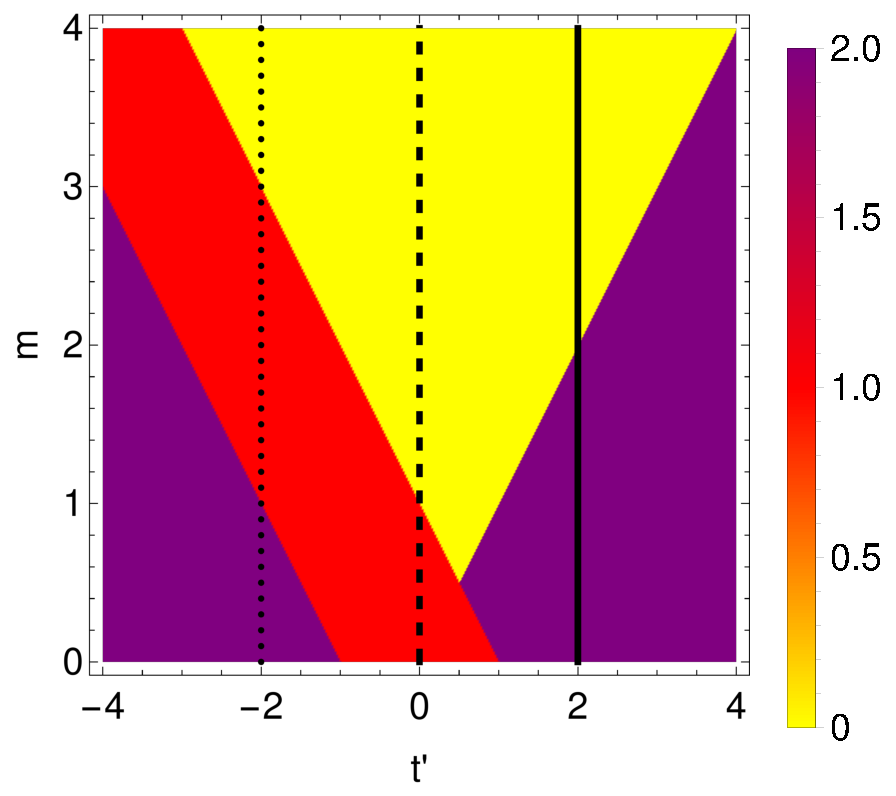
\includegraphics[width=45mm]{phase_diagram2.pdf}
	\caption{Phase diagram for the system in the $BDI$ class showing the winding number of each region. Plotted for parameters $t = 1,\kappa =\kappa'=0.$}
\label{fig:bdi_phase_diagram}
\end{figure}
The BDI class  is characterized by a $\mathbb{Z}$ invariant, the winding number,  in one spatial dimension.
When imposing open boundary conditions on the system, the number of symmetry-protected zero energy edge modes is equal to the winding number. 
The behavior of the  edge modes  is  shown in Fig.~\ref{fig:zero_E_modes}, using the dotted path ($t=1,t'=-2$) marked in the phase diagram. 
Subfigure (a) shows the edge spectrum in the BDI class, with 4 (resp. 2) symmetry-protected zero modes for winding number 2 (1). 
%We also a cut through the three phases (dotted line in the phase diagram) for different values of $\kappa,\kappa'$.  

For $\kappa' \neq 0$ only particle-hole symmetry $C$ is preserved and the system belongs to symmetry class $D$. 
In one spatial dimension, the latter is characterized by a $\mathbb{Z}_2$ invariant.  
Consequently, adding such a term causes the zero modes in the $\nu=2$ phase to split  pairwise and the $\nu = 2$ and $\nu=0$ phases become equivalent. 
This is shown in subfigure (b), where one clearly sees that the zero modes below $m=1$ are split. 

For $\kappa \neq 0$ only time-reversal $T$ is preserved and the system is in the AI class. 
In one dimensions, this class is trivial and, thus,  all zero-energy modes split. 
With both $\kappa \neq 0$ and $\kappa' \neq0$ the system has no local symmetry, thus belonging to the $A$ class.  
Also this symmetry class is topologically trivial in one dimension. 
Subfigures (c) and (d) show the edge spectrum for class AI and A, respectively. In both cases, the edge modes are split from zero for all values of $m$.


%
%In subfigure (b) and (d), where the system is in a topologically trivial phase, all edge modes are gapped. 
%Subfigure (c) shows the edge spectrum of the system being in class D, where the $\nu=2 $ phase becomes trivial. 
%Consequently, symmetry-protected zero modes only exist for $1<m<2.5$\mariac{?} (corresponding to $\nu=1$ for $\kappa'=0$) , whereas the modes are split for $m<1$ (corresponding to $\nu=2$ for $\kappa'=0$).

\begin{figure}[h!]
\centering
%\makebox[0pt]{
%\subfloat[$t = 1,\kappa =\kappa'=0$]{
%  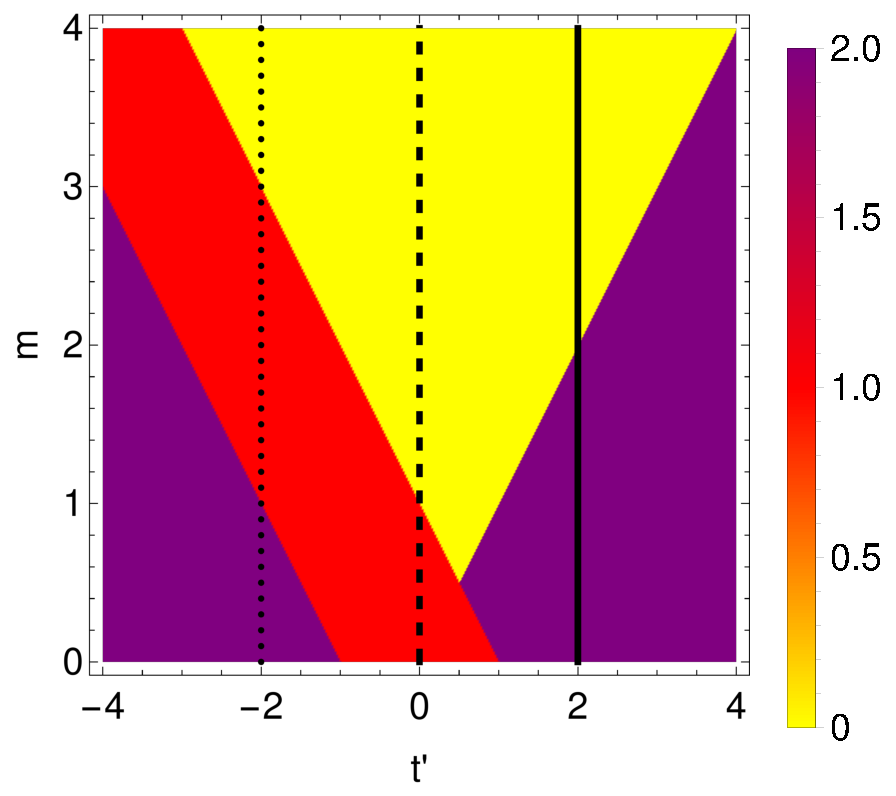
\includegraphics[width=45mm]{phase_diagram2.pdf}
%}}\hspace{0mm}

\makebox[0pt]{
\subfloat[$\kappa =\kappa'=0$]{
  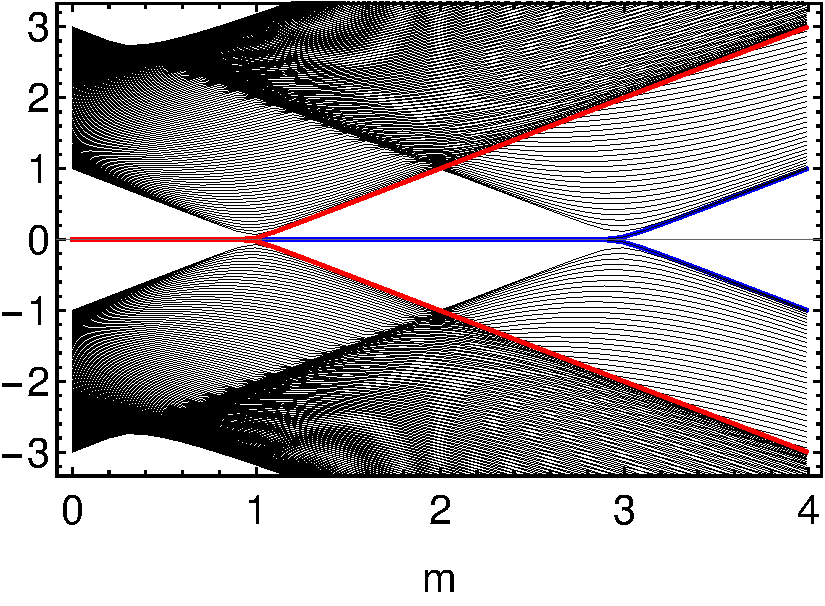
\includegraphics[width=35mm]{2a.pdf}
}
\subfloat[$\kappa = 0, \kappa'=0.3$]{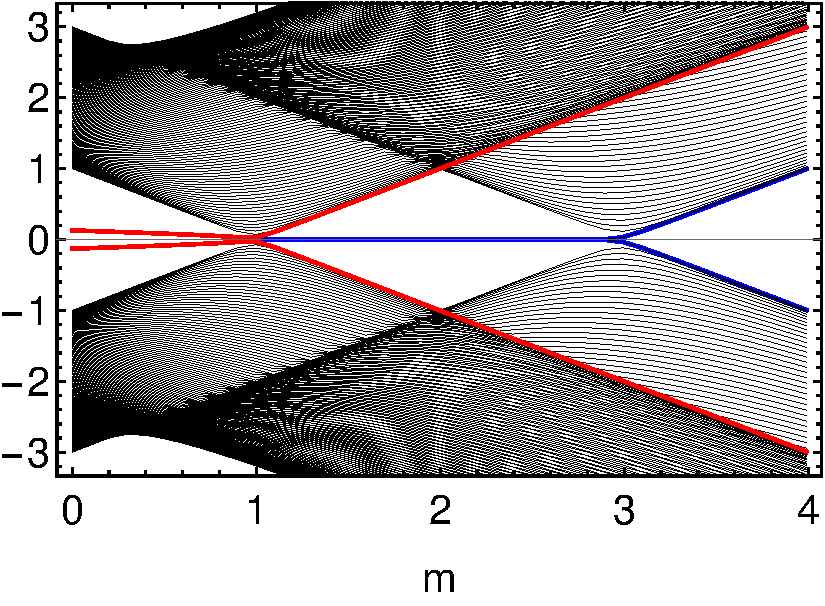
\includegraphics[width=35mm]{2b.pdf}
}
}\hspace{0mm}

\makebox[0pt]{
\subfloat[$\kappa = .3,\kappa'=0$]{
  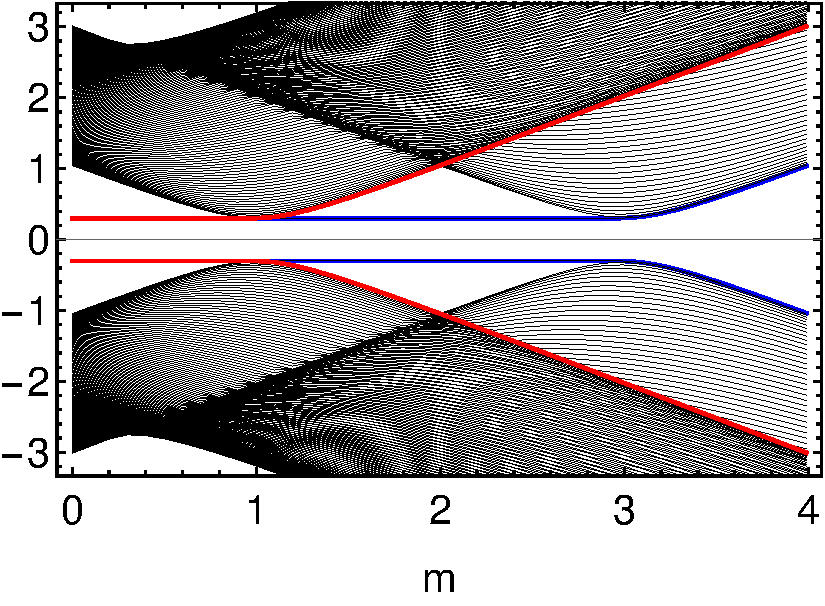
\includegraphics[width=35mm]{2c.pdf}
}
\subfloat[$\kappa = 0.3,\kappa'=0.3$]{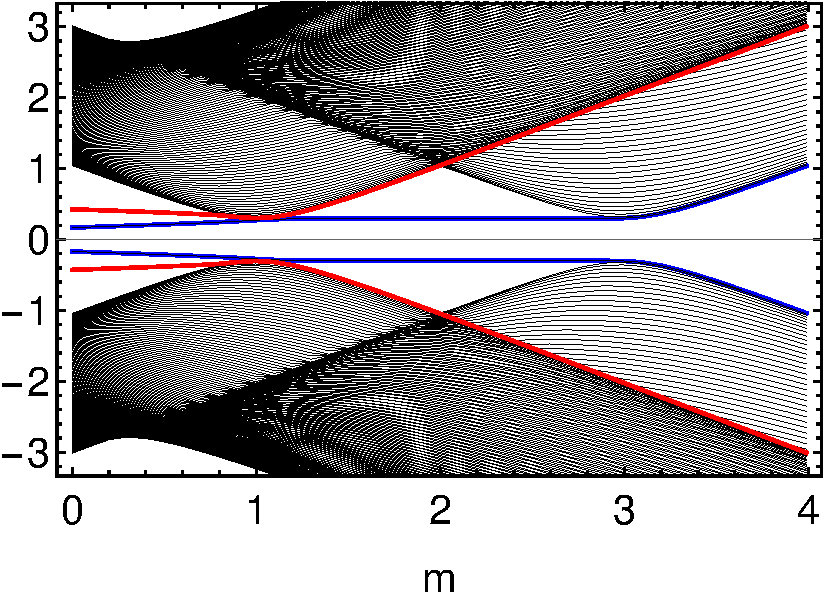
\includegraphics[width=35mm]{2d.pdf}
}
}
\caption{\carlos{Use another colour for the blue edge mode.}Edge spectrum along the dotted path (i.e. $t=1,t'=-2$) of Fig.~\ref{fig:bdi_phase_diagram} for different values of $\kappa$ and $\kappa'$.}
\label{fig:zero_E_modes}
\end{figure}

% - % - % - % - % - % - % - % - % - % - % - % - % - % - % - % - % - % - % - % - % - % - % - % - % - % - % - % - % - % - % - % - % - % - % - % - % - % 
\section{Geometric phases and polarization}

In this section we review some results of the modern theory of polarization, which gave a geometrical description of the polarization \cite{Resta1992,KingSmith1993,Vanderbilt1993,Resta1997} , as well as a recent article by Watanabe and Oshikawa \cite{Watanabe2018} that clarified the meanings of the different polarizations one can define this way and the relations between them. For clarity we will use the same notation they use. 

Consider a generic, quadratic Hamiltonian in one dimension
\begin{equation}\label{eq:quadr_Ham}
\mathcal{H} = \sum_{ij,\alpha\beta} c_{i\alpha}^\dagger H_{ij,\alpha \beta}c_{j\beta}.
\end{equation}
We can obtain its single-particle eigenstates as
\begin{align}
\sum_{j\beta}H_{ij,\alpha\beta} u_{p\mu}^{j\beta} = E_{p\mu} u^{i\alpha}_{p\mu},
\end{align}
where $[U]_{j\beta,p\mu} = u_{p\mu}^{j\beta}$ is the unitary matrix that diagonalizes $H$. In translational invariant systems $u_{p\mu}^{j\beta} = e^{ipj}\tilde{u}_{p \mu}^{\beta}$, where $\tilde{u}_{p \mu}^{\beta}$ are the components of the eigenstates of the Bloch Hamiltonian, $\ket{\tilde{u}_{k\mu}}$. One can now compute the Zak phase \cite{Zak1989}, which for a two-band \mariac{do we need the restriction to two-band models?} model is defined as the geometric phase acquired by the occupied state $\ket{\tilde{u}_k}$ as it winds around the Brillouin zone,
\begin{equation}
\gamma = \int_{0}^{2\pi} dk\, i A_k, 
\label{eq:zak_phase}
\end{equation}
where $A_k = \bra{\tilde{u}_k}\partial_k \ket{\tilde{u}_k}$ is the Berry connection \cite{Berry1984}. The Zak phase is typically regarded as just a phase because it is only gauge invariant modulo $2\pi$. However, for two different states defined by a parameter $\lambda$, as long as $A_k(\lambda)$ is smooth in the path connecting them the change in the Zak phase can be computed as
\begin{equation}
\Delta {\gamma_{\lambda_i \lambda_f}} = \int_{\lambda_i}^{\lambda_f}\int_{0}^{2\pi} dk \, \Omega_{\lambda k},
\label{eq:change_zak_phase}
\end{equation}
where 
\begin{align}\label{eq:BerryCurvature}
\Omega_{\lambda k} = \partial_\lambda A_k(\lambda,k) - \partial_k A_\lambda(\lambda,k)
\end{align}
 is the Berry curvature. The Berry curvature is fully gauge invariant and, therefore, the change in the Zak phase as defined in \eqref{eq:change_zak_phase} is defined along the full real line. The Zak phase itself, as defined above, can be shown to be proportional to the winding number for a certain gauge (see Appendix \ref{appendix:winding_ssh}), which means that it carries physical information beyond modulo $2\pi$. Note that other ways of computing the Zak phase rely on computing $e^{i\gamma}$ instead, such that the result is always defined only modulo $2\pi$.

The derivative of the polarization with respect to some parameter $\lambda$ was obtained \cite{KingSmith1993} as
\begin{equation}\label{eq:Bloch_polarization}
\partial_\lambda \tilde{\mathcal{P}}^{\rm Bloch} = \int_{0}^{2\pi} \frac{dk}{2\pi} \, \Omega_{\lambda k},
\end{equation}
which allows us to make the identification $ \tilde{\mathcal{P}}^{\rm Bloch} = \gamma/2\pi$. As discussed above,  this polarization is defined as an absolute value only modulo 1, however its changes can be defined as a real number. This is no surprise as the derivative of the polarization is related to the current which is a physical observable, unlike $\tilde{\mathcal{P}}^{\rm Bloch}$. 

One can also compute the geometric phase obtained by threading a $U(1)$ flux through the ring \cite{Watanabe2018}, which allows us to compute a polarization in the absence of translational invariance. If the flux is introduced homogeneously through a vector potential $A_x = \Phi/L$ an equivalent polarization can be defined as
\begin{equation}
\mathcal{P} = \int_0^{2\pi}\frac{d\Phi}{2\pi} i\bra{\Psi^\Phi}\partial_\Phi \ket{\Psi^\Phi} + \Im\ln \bra{\Psi^0}e^{2\pi i \hat{P}} \ket{\Psi^{2\pi}}, 
\end{equation}
where $\ket{\Psi^{\Phi}}$ is the ground state in the presence of flux and $\hat{P}=\frac{1}{L}\sum_{j\alpha} j\hat{n}_{j\alpha}$ is the polarization operator. This is equivalent to the polarization obtained by Resta \cite{Resta1997} as
\maria{should I interpret the following line as $\Phi=0$?}
\begin{align}
\mathcal{P} = \frac{1}{2\pi} \rm{ Im }\,\ln\bra{\Psi}e^{2\pi i \hat{P}}\ket{\Psi}.
\end{align}
This expression is particularly useful because it can be easily expressed in terms of single-particle eigenstates as
\begin{align}
\mathcal{P} = \frac{1}{2\pi}\Im \ln \, {\rm det }\!' \, S,
\label{eq:polarization_resta}
\end{align}
where the matrix $S$ is given by
\begin{equation}
S_{p\mu,q\nu} = \sum_{j\alpha} u_{p\mu}^{j \alpha \, \ast} e^{i\frac{2\pi}{L}j}u_{q\nu}^{j \alpha},
\end{equation}
\carlos{I have to check overall sign and sign of exponential.}and  ${\rm det }\!' $ indicates that the determinant is restricted to the space of \emph{occupied} single-particle states. Below we will employ this expression to compare our results with.

There is one last polarization we must consider and it is the one obtained when the flux is introduced in the bond between sites $i=1$ and $i=L$ via twisted boundary conditions. This is equivalent to performing the gauge transformation
\begin{align}\label{eq:Psi_tilde}
\ket{\tilde{\Psi}^\Phi}=e^{i\Phi \hat{P}}\ket{\Psi^\Phi},
\end{align}
which makes $\ket{\tilde{\Psi}_0^\Phi}$ fully periodic in $\Phi$. We can now define the polarization
\begin{equation}
\tilde{\mathcal{P}} = \int_0^{2\pi}\frac{d\Phi}{2\pi} i\bra{\tilde{\Psi}^\Phi}\partial_\Phi \ket{\tilde{\Psi}^\Phi},
\label{eq:p_tilde}
\end{equation}
which is related to the current flowing through the bond \cite{Watanabe2018}. This polarization is related to the homogeneous polarization by 
\begin{equation}
\mathcal{P}= \tilde{\mathcal{P}}+\tilde{\mathcal{P}}_0,
\end{equation} 
where
\begin{equation}
\tilde {\mathcal{P}}_0= \int_0^{2\pi}\frac{d\Phi}{2\pi} \bra{\tilde{\Psi}^\Phi}\hat{P}\ket{\tilde{\Psi}^\Phi}.
\end{equation} 
\maria{Ref to Oshikawa paper?}
%The previous discussion about the Zak phase being defined only modulo $2\pi$ although its changes can be defined as a real number applies in the same way to the polarization obtained in \eqref{eq:p_tilde}.
Note that while $\tilde{\mathcal{P}}$ itself is only defined modulo 1, its changes are again well-defined on the full real axis, similar to the discussion about the Bloch polarization below Eq.~\eqref{eq:Bloch_polarization}. 
In fact, for translationally invariant systems one finds that $\tilde{\mathcal{P}} = \tilde{\mathcal{P}}^{\rm Bloch}$ \cite{Watanabe2018}. 


\section{Entanglement spectrum}
\label{section:ES}
Let us now proceed to discuss the entanglement spectrum. 
An important quantity is the correlation matrix, which in position space is defined by
\begin{align}
C_{ij}^{\alpha \beta} = \expval{c_{i\alpha}^\dagger c_{j\beta}}.
\end{align}
For a system where we occupy all single-particle eigenstates with energies $E<0$ the correlation matrix can be written  as
\begin{align}\label{eq:corr_mat2}
C_{ij}^{\alpha \beta} =& \frac{1}{2}\left[I - H/ (H^2)^{-1/2} \right]_{ij, \alpha \beta}.
\end{align}
This form is particularly useful for all our subsequent calculations, since it does not require diagonalizing the Hamiltonian.

In this manuscript, we are mainly interested in the spectrum of the correlation matrix, when restricted to a spatial sub-region $A$ (its complement will be denoted by $B$ in the following). 
Following Ref.s~\cite{Huang2012,Huang2012-2}, we refer to this spectrum as the entanglement occupancy spectrum (EOS). 
The resulting eigenvalues  are denoted by $\xi_j$. 
%We will differentiate between two types of eigenvalues: those (exponentially) close to $\xi_j=0 (1)$ correspond to ``bulk'' states, by which we mean that the corresponding eigenstates lie (up to exponentially small corrections) in  $A$ ($B$). 
%Values $0<\xi_{l,r}<1$ indicate states that are located at the virtual boundaries -- labeled `left' and `right' in the following-- between $A$ and $B$~\cite{Peschel2008}. 
%There is, of course, an ambiguity here on dividing eigenstates of the EOS into ``bulk'' and ``edge'' states and `how close' the eigenvalue has to be to $0,1$ in order to qualify as a bulk state. 
%XXXX
Topological phases are characterized by (symmetry-protected) zero-energy modes in the edge spectrum and $\xi=\frac 1 2$ modes in the EOS~\cite{Fidkowski2010entanglement}.
 

The EOS is in one-to-one correspondence to the entanglement spectrum (ES). 
Following Ref.~\cite{Peschel2003}, one can write the  reduced density matrix as 
\begin{align}\label{eq:red_dens_mat}
\rho_A&=\mathcal{K} \exp(-\mathcal H),
\end{align}
where $\mathcal{K}$ is a normalization constant and $\mathcal{H}$ is a quadratic Hamiltonian, referred to as entanglement Hamiltonian. 
The eigenvalues $\epsilon_j$ of $\mathcal{H}$, referred to as entanglement energies,  are related to the EOS by 
\begin{align}\label{eq:xi_eps}
\xi_j &=\left(e^{\epsilon_j}+1\right)^{-1}, 
\end{align}
the corresponding eigenstates are the same. 
Eq.~\eqref{eq:xi_eps} implies that the full information of the \emph{many-particle} ES is contained in the single-particle spectrum of the reduced correlation matrix. 
The latter is much simpler to interpret. 
Consequently, we will focus on the EOS in the remainder of the manuscript and only mention the ES when necessary. 

One property of the subsystem correlation matrix we will make use of later is that, for sufficiently large systems, its eigenstates are found to be localize on either virtual edge if $\xi \neq 0,1$, or they are found to be bulk modes if the correspondent eigenvalues are exponentially close to $\xi = 0,1$ \cite{Peschel2008}.

%The single-particle entanglement spectrum (ES) is then obtained as the spectrum of the subsystem correlation function obtained after bisecting the system into two equal parts. 

%In the ES we can differentiate between two types of eigenvalues, which we denote by $\xi$. The ones at $\xi_b = 0,1$ correspond to bulk states while for the ones in between, $0<\xi_{l,r}<1$, we find their correspondent eigenstate localized in either the left, $\xi_l$, or right, $\xi_r$, virtual edge \cite{Peschel2008}. 
%\mariac{introduce entanglement energy, relation between C and energies}


A few comments are needed regarding  bipartition. 
In the following sections, we show how the Zak phase can be recovered from the EOS.
We also give a simple formula that is identical to the Zak phase in the thermodyamic limit.  
However, for a generic, finite size system, there will be finite-size discrepancies between our formula and the Zak phase.
In order to reduce these, we are going to choose $A$ as half the system in the remainder of the manuscript.
The results (in the thermodynamic limit) do not depend on this choice. 
% - % - % - % - % - % - % - % - % - % - % - % - % - % - % - % - % - % - % - % - % - % - % - % - % - % - % - % - % - % - % - % - % - % - % - % - % - % 
\section{Zak phase in the EOS}

Let us first review previous results on the relation between the entanglement spectrum and the Zak phase. 
For symmetry-protected topological systems in one dimension, the quantized Zak phase is zero whenever there is an even number  of eigenvalues per edge at $\xi = 1/2$, and $\pi$ when the number is odd~\cite{Peschel2008}. 
Ryu and Hatsugai considered the fully dimerized SSH chain with broken chiral symmetry~\cite{Ryu2006}.  
This model is rather special in that there is only a single pair of eigenvalues, related by symmetry, in the EOS that is not identical to $0$ or $1$. 
In fact, the authors could show that the value of one of these `midgap states' is identical to the Zak phase divided by $2\pi$, or $\tilde{\mathcal{P}}^{\rm Bloch}$. 
Their result is a particular limit of Eq.~\eqref{eq:chi_integrable}. 
%
%Beyond symmetry protected systems, there was observed that in the fully dimerized SSH chain, with only a single mode present in the ES, the Zak phase is equal to the midgap eigenvalue \cite{Ryu2006}. 
Huang and Arovas considered a two-dimensional chern insulator and noted that the Zak phase qualitatively follows the `virtual edge mode' that connects the EOS values at 0 to those at 1~\cite{Huang2012,Huang2012-2}. 
Interpreting this as a one-dimensional system with a parameter, we can explain this behavior by Eq.~\eqref{eq:chi_integrable}, noting that there is a single pair of eigenvalues that dominates the sum. 
Note that the observation of Ref.s~\cite{Huang2012,Huang2012-2} is particular to a system with Chern number 0 or $\pm 1$, and it generically fails for systems with higher Chern numbers. 
In the latter case, there are several terms in Eq.~\eqref{eq:chi_integrable} with comparably large contributions. 
%For cases with more edge modes present in the ES it has been shown that the Zak phase follows the midgap eigenvalues qualitatively \cite{Huang2012,Huang2012-2}. 


\subsubsection{Systems with equidistant entanglement energies}
\mariac{add scaling plot for $\chi$ versus $\gamma/(2\pi)$. }
We first discuss systems, for which the entanglement energies of a \emph{single} virtual edge are equidistant. This is a feature of integrable systems \cite{Peschel1999} for e.g. nearest neighbor hopping models such as the SSH chain, and applies to the Hamiltonian~\eqref{bdi_model} when $t'=0$. 
In this case, one can obtain the Zak phase in a very simple fashion: We reorder the eigenvalues of the ES by magnitude, $\xi_1 < \xi_2 < ...< \xi_{L_AM}$, and compute
\begin{equation}
\chi = \sum_{j=1}^{L_A M/2} \xi_{2j-1} \, {\rm mod} \, 1.
\label{eq:chi_integrable}
\end{equation}
In the thermodynamic limit, $\chi$ becomes identical to either $\tilde{\mathcal{P}}^{\rm Bloch}$ or $1-\tilde{\mathcal{P}}^{\rm Bloch}$
\begin{equation}
\lim_{L \rightarrow \infty} \abs{\tilde{\mathcal{P}}^{\rm Bloch}} = \lim_{L \rightarrow \infty} \abs{\chi}.
\end{equation}
For translational invariant systems the EOS is symmetric such that a crossing of the eigenvalues $\xi$ results in $\chi$ changing sign. This is particularly irrelevant in the case of symmetry-protected states where the Zak phase is quantized to $0$ or $\pi$. 

In the case where there is only one eigenvalue per edge that is $\neq 0,1$ in  the EOS, like in the fully dimerized limit of the SSH chain, we recover the equality between the midgap eigenvalue and the Zak phase found in Ref.~\cite{Ryu2006}. 

In Fig.~\ref{huang} we show  the EOS along the dashed cut in the phase diagram of Fig.~\ref{fig:bdi_phase_diagram}. 
Along this line, our model is equivalent to an SSH chain. 
In the presence of chiral and translation symmetry, all eigenvalues of the EOS are doubly degenerate --- one eigenvalue from each edge, such that $\chi$ from \eqref{eq:chi_integrable} will pick up one eigenvalue from each pair. Because of chiral symmetry the sum of the two eigenvalues related by the symmetry gives always $1$ so they do not contribute to $\chi$. The only contribution to $\chi$ is the one from the eigenstates with $\xi=1/2$ that do not have a chiral partner, see Fig.~\ref{huang}(a). Here we see explicitely the known relation between the Zak phase and the number of $\xi = 1/2$ modes.

Note that the full sum~\eqref{eq:chi_integrable}  evaluates to zero in the trivial regime %up to finite-size corrections% \carlos{It is actually exact due to symmetry}.
despite the presence of modes with entanglement occupancy $0<\xi<1$. 

When breaking chiral symmetry, the EOS will no longer be doubly degenerate. 
For small $m$, there are two dominant midgap eigenvalues, and the Zak phase follows the lower one very closely, see Fig.~\ref{huang}(b).
When this midgap eigenvalue approaches  0, the contribution from the other modes becomes more relevant and the Zak phase starts to deviate from the midgap eigenvalue, \mariac{see inset}.
\begin{figure}[t]
\centering
\makebox[0pt]{
\subfloat[$t = 1,t'=0$, \, \,$\kappa =\kappa'=0$]{
  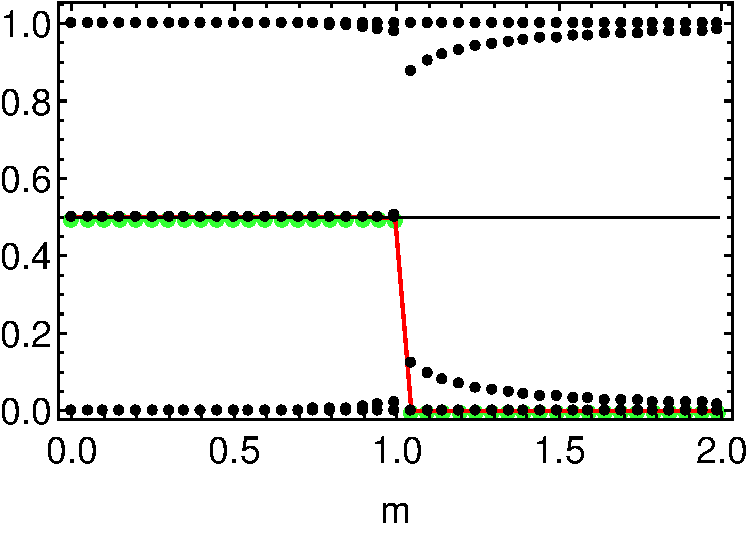
\includegraphics[width=35mm]{2_a.pdf}
}
\subfloat[$t=1,t'=0$, $\kappa = 0.3, \kappa'=0$]{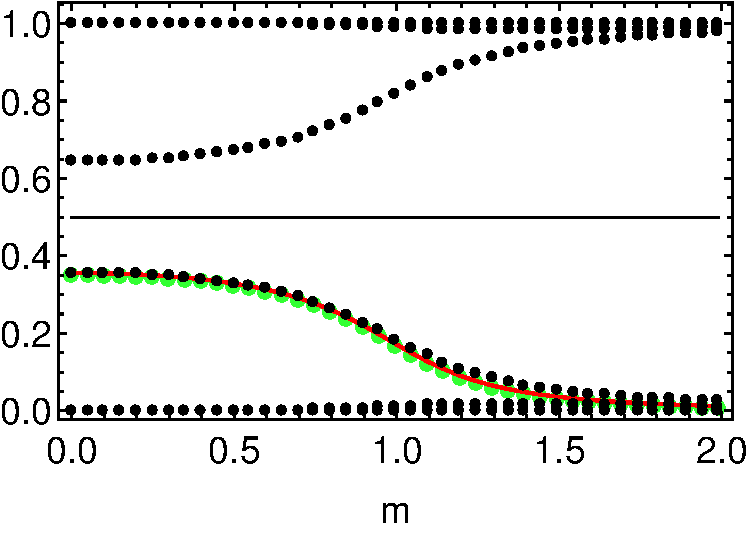
\includegraphics[width=35mm]{2_b.pdf}
}
}
\caption{Entanglement spectrum (black), $\chi$ (green) and $\frac{\gamma}{2\pi}$ (red) for a cut in the phase diagram through the $\nu = 1 \rightarrow \nu = 0$ transition (dashed line in~\ref{fig:bdi_phase_diagram}
	) for $t'=0$ and different values of $\kappa$. Computed for $L=40$.}
\label{huang}
\end{figure}

\subsubsection{General case}

In general we find that it is only the eigenstates that localize on the left edge that should contribute to $\chi$. The inclusion of bulk modes is irrelevant since they have $\xi = 0,1$. We can then compute the average position of each eigenstate and construct $\chi$ from the eigenstates with $\expval{\hat{x}}<L/4$, with $L/4$ being the middle point of region $A$,
\begin{equation}
\chi = \sum_{\mu \in A_L} \xi_\mu \, {\rm mod} \, 1. 
\label{eq:chi_left}
\end{equation}
In the thermodynamic limit, it is $\tilde{\mathcal{P}}$ that we actually identify with $\chi$
\begin{equation}
\lim_{L \rightarrow \infty} \tilde{\mathcal{P}} = \lim_{L \rightarrow \infty} \chi.
\label{eq:ptilde_eq_chi}
\end{equation}
Note that in order to compute $\chi$ correctly the eigenstates with $\xi \neq 0,1$ need to be localized in order for us to select the correct eigenvalues. It might be --- like in Fig.\ref{huang}(a) --- that the spectrum has degenerate pairs of left and right eigenstates and the numerical diagonalization mixes them. This case is trivial, as we know that there is one left and one right eigenstate but if the degeneracy is four-fold or higher one needs to obtain the localized eigenstates. Localizing the eigenstates that are exponentially close to $\xi = 0,1$ is more difficult but not doing so only results in an exponentially small error. 

Before proceeding lets review again the result in the previous section. First note that for translation invariant systems, the ES of the right and the left edge are related by an overall '-' sign, i.e. for each eigenvalue $\epsilon$ on the right edge, there is a corresponding value $-\epsilon$ on the left edge. 
Since the spectra are equidistant, this implies that the two edge spectra are merely shifted with respect to each other.
If the shift is zero, e.g.  in presence of a symmetry, summing every other eigenvalue is equivalent, modulo 1, to summing all the left eigenvalues. With a finite shift summing all odd eigenvalues corresponds to either summing all left eigenvalues or all right eigenvalues. In general, it implies that $\chi$ as defined in Eq.~\eqref{eq:chi_integrable} only gives the Zak phase up to an overall sign. This issue can be fixed by determining the localization of a single eigenstate. 
\begin{figure}[t]
	\centering
	\makebox[0pt]{
		\subfloat[$t = 1, t' = 2,$   $\kappa =0.3, \kappa' = 0$]{
			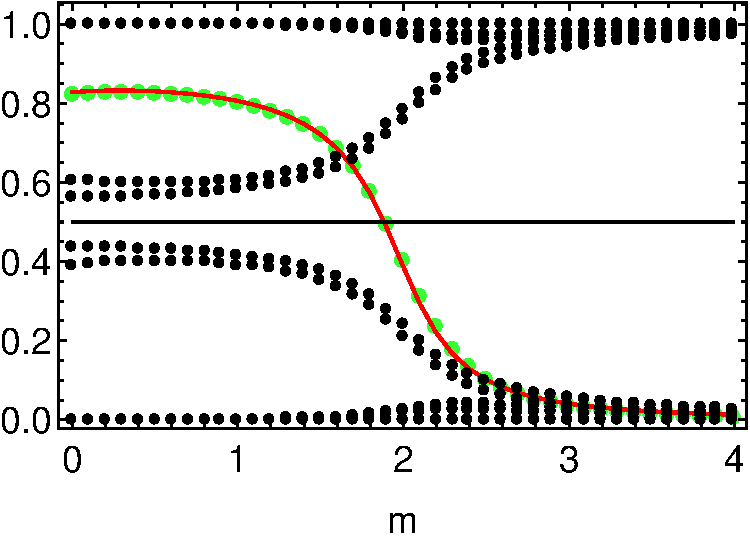
\includegraphics[width=35mm]{3_a.pdf}
		}
		\subfloat[$t = 1, t' = 2,$ $\kappa = 0, \kappa' = 0.3$]{
			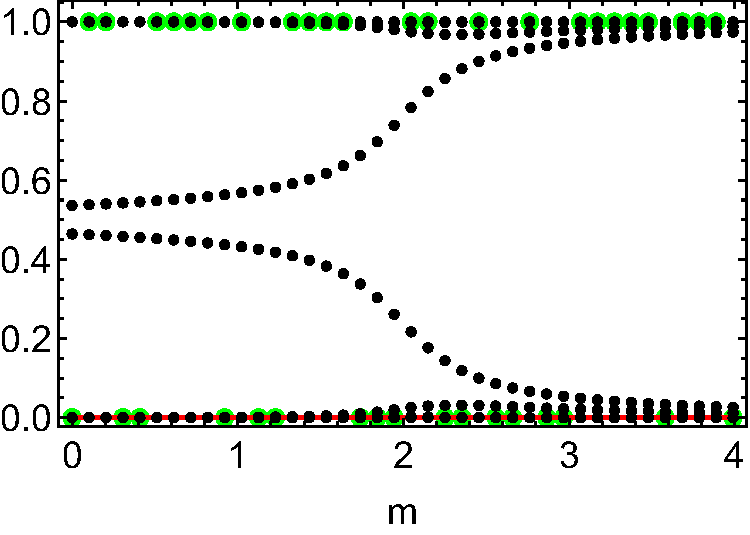
\includegraphics[width=35mm]{3_b.pdf}
		}
	}\hspace{0mm}
	
	\makebox[0pt]{
		\subfloat[$t = 1, t' = -2,$ $\kappa = 0.3, \kappa' = 0$]{
			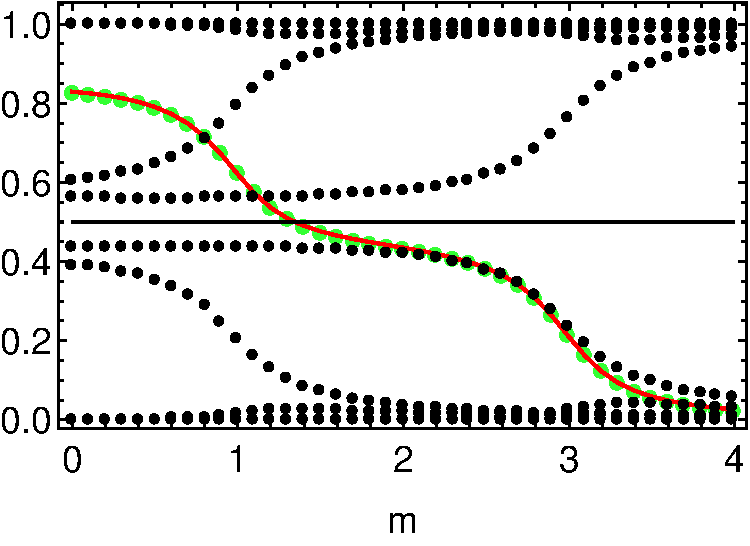
\includegraphics[width=35mm]{3_c.pdf}
		}
		\subfloat[$t = 1, t' = -2,$ $\kappa = 0, \kappa' = 0.3$]{
			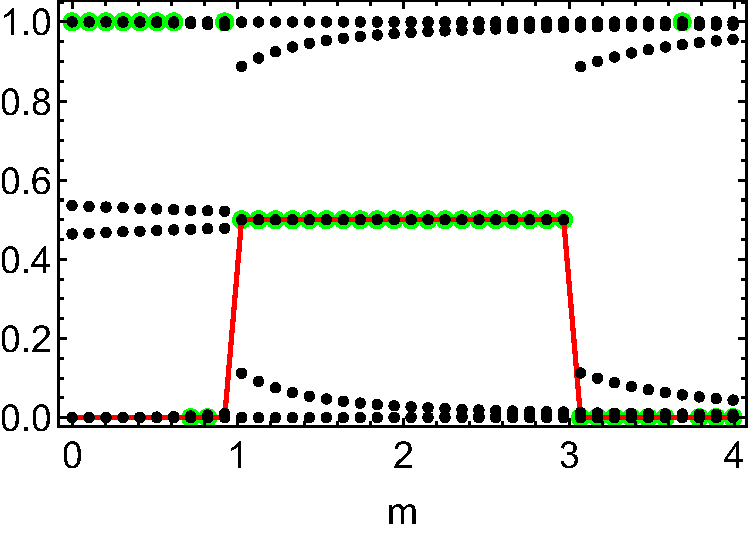
\includegraphics[width=35mm]{3_d.pdf}
		}
	}\hspace{0mm}
	
	\makebox[0pt]{
		\subfloat[$t = 1, t' = -2,$ $\kappa_i \neq 0 , \kappa' = 0$]{
			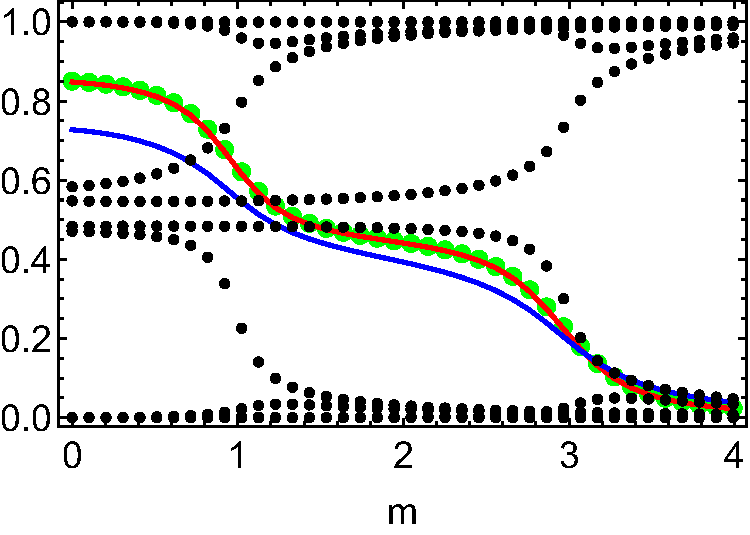
\includegraphics[width=35mm]{3_e.pdf}
		}
	}
	\caption{(a,b,c,d) Entanglement spectrum (black), $\chi$ (green) and $\tilde{\mathcal{P}}$ (red) for two different cuts with both $\kappa$ and $\kappa'$ symmetry breaking terms. Note that in this case where there is translational invariance $\tilde{\mathcal{P}}=\tilde{\mathcal{P}}^{\rm Bloch}$, which is nothing else than the Zak phase over $2\pi$. (e) Same as (c) but with a position dependent $\kappa_i=(i+L/4 \, {\rm mod}\, L)/L$. We also plot $\mathcal{P}+1/2$ (blue) to showcase that $\chi$ is indeed equal to $\tilde{\mathcal{P}}$ and not $\mathcal{P}$ as in the translationally invariant case $\tilde{\mathcal{P}}=\mathcal{P}+(L+1)/2$. }
	\label{2}
\end{figure}

In Fig.\ref{2} we show two examples that highlight the importance of the localization structure of the EOS. 
In subfigures (a) and (b), we compute the EOS for varying $m$ at  $t=1$, $t'=2$, indicated by the solid line  in the phase-diagram in Fig.~\ref{fig:bdi_phase_diagram}, in the presence of two different symmetry breaking terms: (i) $\kappa =0.3$, $\kappa'=0$ and (ii) $\kappa=0$, $\kappa'=0.3$.  
For $\kappa=\kappa'=0$, there is a phase transition $\nu = 2 \rightarrow 0 $ at $m=2$, whereas both choices of symmetry breaking render the system trivial  for all $m$.
However, the two symmetry breaking terms split the four-fold degenerate $\xi=1/2$ midgap states very differently, thus resulting in completely different Zak phases despite the superficial resemblance of their respective EOS.  
While $\kappa'$ splits the four-fold degenerate states into two two-fold degenerate pairs at opposite edges whose contribution cancels (modulo 1), $\kappa$ split them into two $left-left$ and $right-right$ pairs, with a finite contribution to the Zak phase. 
In subfigures (c) and (d), we consider the same symmetry breaking terms, but now for $t=1$ and $t'=-2$, where the BDI systems shows a phase transition  $\nu=2\rightarrow 1\rightarrow 0$. 
Note that the $\kappa'$ term does not render the $\nu=1$ phase trivial, and the Zak phase will remain quantized in that region, see Fig.~\ref{2}(d). 
Also here, Eq.~\ref{eq:chi_left} correctly reproduces the Zak phase for all values of $m$. 
Note that in all examples shown in this subsection, the observations made in references \cite{Huang2012,Huang2012-2}, i.e. that the behavior of the Zak phase resembles that of the entanglement occupancy midgap states, do not apply anymore. 

Since $\chi$ is naturally defined in position space it is also valid for systems without translationally invariance. We show this in Fig.\ref{2}(e) where we show the EOS, $\chi$, $\mathcal{P}$ and $\tilde{\mathcal{P}}$ along the dotted cut in the phase diagram with an added position dependent symmetry breaking term $\kappa_i = (i+L/4 \, {\rm mod}\, L)/L$ (\carlos{I added this profile because with disorder $\tilde{\mathcal{P}}$ and $\mathcal{P}$ are difficult to distinguish}). We obtain that $\chi$ is indeed identified with $\tilde{\mathcal{P}}$ as we hinted at before, and not $\mathcal{P}$, although these two polarization only differ by $(L+1)/2$ in the translationally invariant case. 


This relation between the Zak phase and the EOS is a consequence of an identity between the Zak phase and the many-body entanglement spectrum previously found for infinite chains \cite{Zaletel2014}. In Appendix A we modified this derivation to account for the periodic boundary conditions we use and show how their result simplifies greatly when expressing it in terms of the EOS, resulting in.~\eqref{eq:ptilde_eq_chi}.



% - % - % - % - % - % - % - % - % - % - % - % - % - % - % - % - % - % - % - % - % - % - % - % - % - % - % - % - % - % - % - % - % - % - % - % - % - % 

\section{Chern number and Winding number}


In Appendix A we obtain that $\chi$ should be the sum of all the eigenvalues of eigenstates related to the cut between $i=1$ and $i=L$ that make a subspace $A_L$. The dimension of $A_L$ is however not well-defined as one can always include bulk modes into it. Since the bulk modes have $\xi = 0,1$ this makes $\chi$ well-defined only modulo 1. This can be avoided by computing instead
\begin{equation}\label{eq:tpo}
\tpo = \int_0^{2\pi}\frac{d\Phi}{2\pi} i\brapsio{\Phi}\partial_\Phi \ketpsio{\Phi}.
\end{equation}
where $\ketpsio{{\Phi=0}}$ is the ground state of the chain opened between sites $i=L/2$ and $i=L/2+1$ and 
\begin{equation}
\ketpsio{\Phi} =e^{-i \Phi \hat{N}_A} \ketpsio{0}.
\label{eq:gauge}
\end{equation}
The difference with the closed chain being that now there is no ambiguity on when an electron crosses the boundary with the twisted boundary condition. Note that since the chain is open, $\Phi$ is not a flux but should now be regarded as a parameter and therefore $\tpo$ does not need to be a physical polarization.  $\tpo$ can be obtained in an even simpler way than $\tilde{\mathcal{P}}$ as 
\begin{align}\label{eq:phi_independence}
\tpo =&  \int_0^{2\pi}\frac{d\Phi}{2\pi} \brapsio{0} \hat{N}_A \ketpsio{0} \nonumber \\
=&\sum_{\alpha,j\in A}\brapsio{0} c_{j\alpha}^\dagger c_{j\alpha} \ketpsio{0} \nonumber\\
=&\sum_{\alpha,j\in A} C_{\rm o,j\alpha,j\alpha}\nonumber \\
=& {\rm Tr}[C_{A,\rm o}],
\end{align}
where we used Eq.~\eqref{eq:gauge} and $C_{\rm o}$($C_{A,\rm o}$) denotes the (reduced) density matrix of the open chain. 
Note that Eq.~\eqref{eq:phi_independence} is nothing else than the generalization of $\chi$ to the open chain. 
\maria{I am not entirely happy with the following argument, as it goes wrong in the topological phase. We mention this later, but we should already mention it here. }
The idea is that in the process of opening the chain, which can be done adiabatically, all eigenvalues that are not in $A_L$ should get pushed to $\xi=0$ or $\xi=1$. 
If for a given path in parameter space $\boldsymbol{\lambda}_i \rightarrow \boldsymbol{\lambda}_f$ their contribution remains constant, that is, there are no jumps between $\xi=0$ and $\xi=1$ and $\tpo (\boldsymbol{\lambda} )$ is smooth, then changes in $\tpo(\boldsymbol{\lambda}_i ) $ along the path will be defined as a real number and not only modulo 1. Since $\tilde{\mathcal{P}}$ is a local property of the bond between $i=1$ and $i=L$ one would expect it to not depend on what happens far from it such that $\tpo$ and $\tilde{\mathcal{P}}$ are equivalent. 

\subsubsection{SSH chain}

Consider the simple case of the SSH chain, with $t'=0$ in the model. In the chiral symmetric case, $\kappa = 0$, the open chain presents zero-energy modes for $m<t$ that seem problematic. $\tilde{\mathcal{P}}_{\rm open}$  will depend on the occupation of these zero modes although we just argued that $\tilde{\mathcal{P}}$ should not, since the zero-energy modes are localized far from the virtual cut at $i=1$. We can break the chiral symmetry in order to split the zero-energy modes so we do not have to make this choice, but the resulting $\tilde{\mathcal{P}}_{\rm open}$ will be discontinuous at $\kappa = 0$, suggesting that the limit does not exist. This can be seen from the fact that the Hamiltonian now has the symmetry
\begin{equation}
SH(\kappa)S = -H(-\kappa), \quad S C_A(\kappa) S = \mathbb{I}-C_A(-\kappa)
\end{equation}
so $\tpo(-\kappa) = L-\tpo(\kappa)$. Unless $\tpo(0) = L/2$, which only happens in the trivial case, the result will be discontinuous at $\kappa = 0$. We can see this in Fig.\ref{ssh_chern}.(a) where we show $\tpo$ in the space $(m,\kappa)$. This branch cut is in fact not an artifice of the open chain trick, but the result of the degenerate point at $(m=t,\kappa=0)$ having an associated Chern number $C=1$ \cite{Asboth2016}.

Consider a loop around the singularity at $(m=t,\kappa=0)$ parametrized by $\theta$. The Chern number is then defined as
\begin{equation}
C = \int_0^{2\pi}d\theta\int_0^{2\pi}\frac{d\Phi}{2\pi} \Omega_{\theta\Phi},
\label{eq:chern}
\end{equation} 
with the Berry curvature $\Omega_{\theta\Phi}$ defined in Eq.~\ref{eq:BerryCurvature}. 
From  Eq.~\eqref{eq:tpo}, it follows that the Berry connection for the flux is simply $A_\Phi(\theta,\Phi,) = -i\tpo(\theta)$, so we only need to compute $A_\theta(\theta,\Phi)$. (\carlos{Please double check this calculation}) Expanding $\ketpsio{\Phi}$ in the eigenbasis of the number operator $\hat{N_A}$ -- denoted by $\{\ket{j}\}$ -- we can compute its derivative with respect to the parameter $\theta$ as
\changed{changed}
\begin{align}
\partial_\theta \ketpsio{\Phi} =& \sum_j [\partial_\theta c_j (\theta)]e^{-i\Phi N_A^j}\ket{j}.
\end{align}
where $c_j(\theta) = \Big\langle j\ketpsio{0}$ does not depend on $\Phi$. The correspondent Berry connection then gives
\begin{align}
\brapsio{\Phi}\partial_\theta \ketpsio{\Phi} =& \sum_{lj} c^*_l(\theta) [\partial_\theta c_j(\theta)] \bra{l} e^{i\Phi (N_A^lN_A^j)}\ket{j}\nonumber\\
=& \sum_j  c^*_j(\theta) \partial_\theta c_j(\theta) \nonumber\\
=&\brapsio{0}\partial_\theta \ketpsio{0}, 
\end{align}
i.e. it is independent of $\Phi$. 

The integral in \eqref{eq:chern} is performed on the surface of the torus defined by $(\theta,\Phi)$. Because the Berry connection $A_\Phi(\theta)$ is not smooth one cannot directly apply Stokes theorem. Instead, consider that we split the torus in two cylinders, $S_1$ with $\theta\in[\theta_0,2\pi-\theta_0]$ and  $S_2$ with $\theta\in[2\pi-\theta_0,2\pi+\theta_0]$ and we change the gauge in $\boldsymbol{A}(\theta)$ such that it is smooth in each cylinder. We can now apply Stokes theorem to the two cylinders independently
\begin{align}
C_1 =& \int_{S_1} d\boldsymbol{S}\cdot (\nabla \times \boldsymbol{A}) \nonumber\\
=& \int_{\partial S_1} d\boldsymbol{l}\cdot \boldsymbol{A}(\theta,\Phi) \nonumber\\
=& \int_a^{2\pi-a} d\theta A_\theta(\theta,0) +\int_0^{2\pi} \frac{d\Phi}{2\pi} A_\Phi (2\pi-a,\Phi) \nonumber\\
&-\int_a^{2\pi-a} d\theta A_\theta(\theta,2\pi) -\int_0^{2\pi} \frac{d\Phi}{2\pi} A_\Phi (a,\Phi).
\end{align}
In our case, $A_\theta$ is independent of $\Phi$ so the terms involving it cancel and we have
\begin{align}
C_1 =& \int_0^{2\pi} \frac{d\Phi}{2\pi} [A_\Phi (2\pi-a,\Phi) -A_\Phi (a,\Phi)].
\end{align}
Similarly computing the integral for the other cylinder we obtain
\begin{align}
C_2 =& \int_0^{2\pi} \frac{d\Phi}{2\pi} [A'_\Phi (2\pi+a,\Phi) -A'_\Phi (2\pi-a,\Phi)].
\end{align}
The Chern number is then $C=C_1+C_2$. Noting again that $A'_\Phi(\theta)$ is continuous in $S_2$ taking the limit of $a\rightarrow 0^+$ makes $C_2$ vanish and the Chern number is given by
\begin{align}
C =& \int_0^{2\pi} \frac{d\Phi}{2\pi} [A_\Phi (2\pi^-,\Phi) -A_\Phi (0^+,\Phi)].
\end{align}
If we consider the loop starting at $\kappa = 0$ this is exactly the case shown in Fig.\ref{ssh_chern}.(a), where $A_\Phi (\theta,\Phi) = \tilde{\mathcal{P}}_{\rm open}(\theta)$ is smooth everywhere but in $\theta = 0$, and therefore we can compute the Chern number simply as 
\begin{align}
C= \tpo(\kappa=0^+)-\tpo(\kappa=0^-).
\end{align}
Using the symmetry of the polarization described above this results in 
\begin{align}
C= 2\tpo(0^+)-L.
\label{eq:Chern_number}
\end{align}
The discontinuity in $\tpo$ is therefore related to the Chern number.% and it is not merely continuous modulo 1. 

One can also obtain a polarization continuous in $\kappa$ by doing a gauge transformation 
\begin{align}
\ket{\tilde{\psi}^{\prime \,\Phi}}=e^{ i \Phi \Theta(-\kappa)\Theta(t-m)}\ket{\tilde{\psi}^{\Phi}}
\end{align}
\maria{where $\Theta$ is the Heaviside theta function (?)}. 
This gauge transformation places the branch cut at $m=t,\kappa < 0$, as can be seen in Fig.\ref{ssh_chern}(b)  (\carlos{need to double check signs}). 
This is in fact the result one gets when using the gauge that allows one to compute the winding number from the Zak phase. \maria{???}

%\changed{undo figure uncomment}
\begin{figure}[t]
	\centering
	\makebox[0pt]{
		\subfloat[$\tilde{\mathcal{P}}_{\rm open}-L/2$]{
			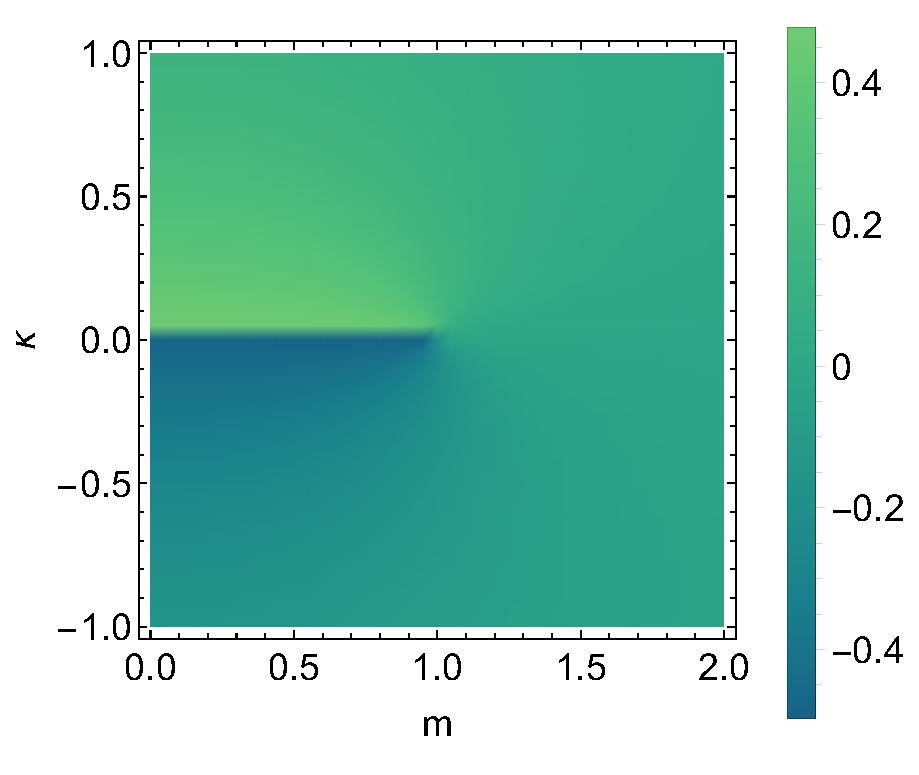
\includegraphics[width=50mm]{windingSSH1.pdf}
		}
		\subfloat[$\tilde{\mathcal{P}}_{\rm open,+}-L/2$]{
			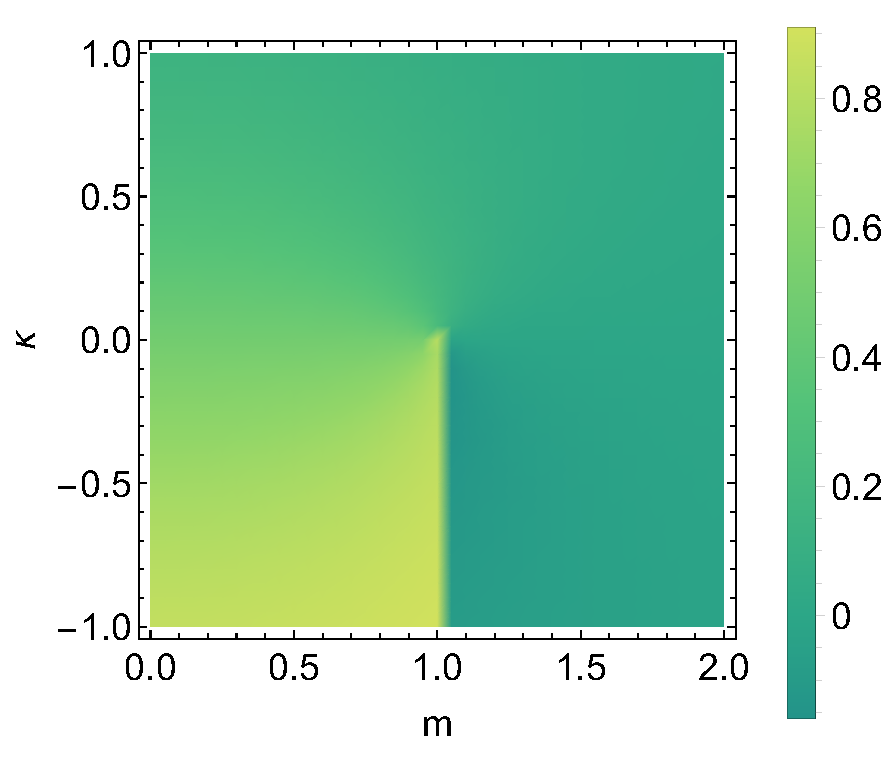
\includegraphics[width=45mm]{windingSSH2.pdf}
		}
	}\hspace{0mm}
	
	\makebox[0pt]{
		\subfloat[$\tilde{\mathcal{P}}_{\rm open}-L/2$]{
			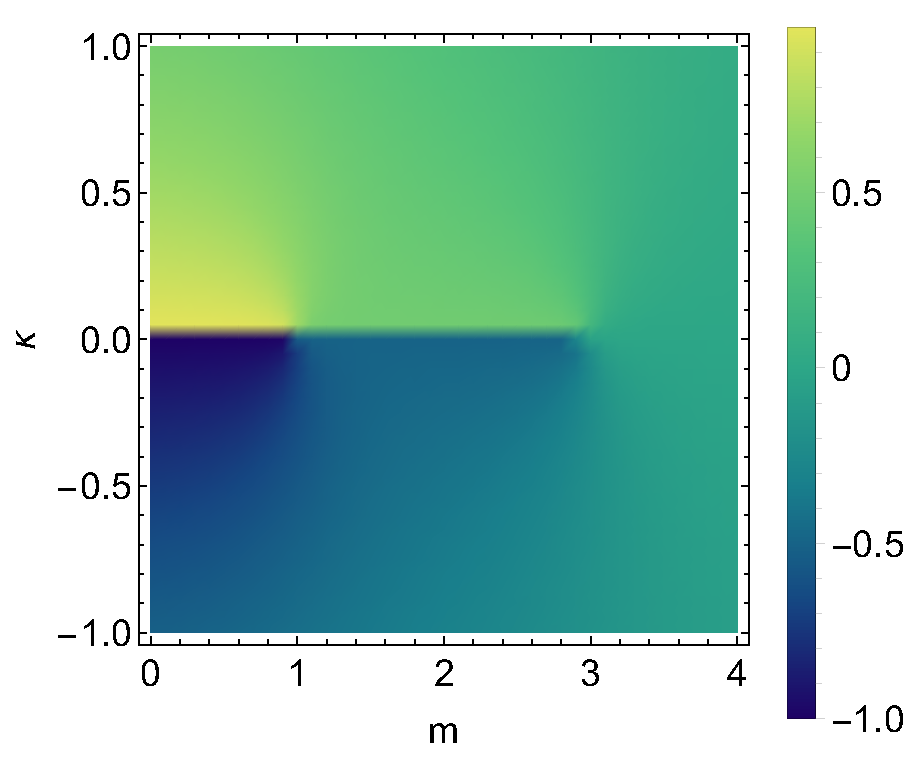
\includegraphics[width=45mm]{windingtp1.pdf}
		}
		\subfloat[$\tilde{\mathcal{P}}_{\rm open,+}-L/2$]{
			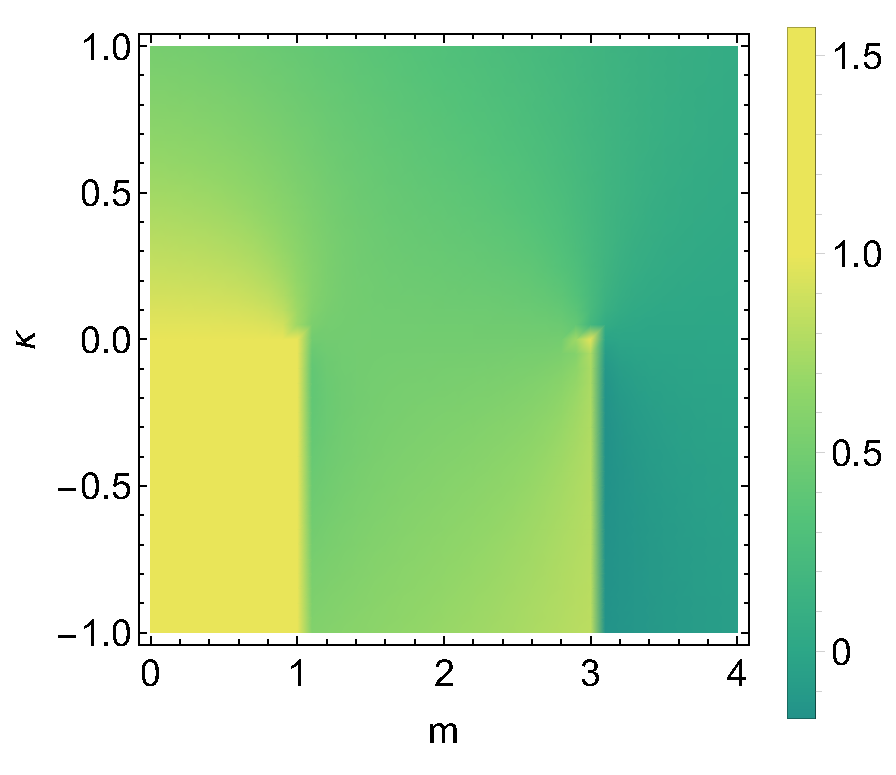
\includegraphics[width=45mm]{windingtp2.pdf}
		}
	}
	\caption{Polarization $\tilde{\mathcal{P}}_{\rm open}$ computed for three different gauge choices, for $t=1,\kappa'=0$ and system size $L=160$. (a) and (b) with $t'=0$ and (c) and (d) for $t'=-2$. }
	\label{ssh_chern}
\end{figure}

%\changed{undo figure uncomment}

\begin{figure}[t]
	\centering
	\makebox[0pt]{
		\subfloat[$\tilde{\mathcal{P}}_{\rm open}$]{
			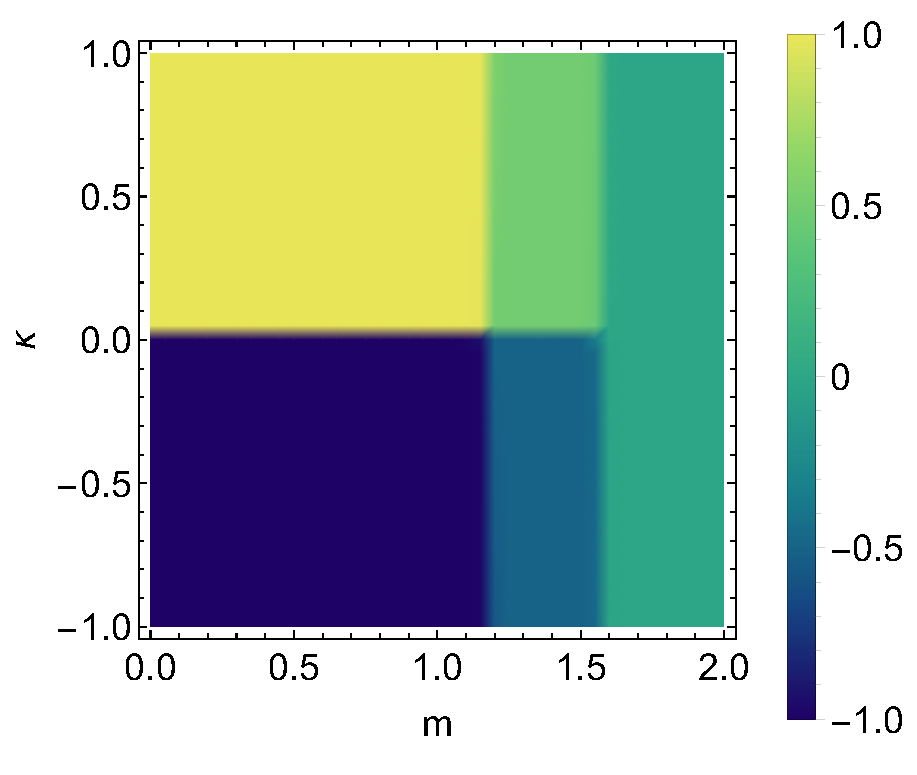
\includegraphics[width=50mm]{windingtpdis.pdf}
		}
		\subfloat[$C $]{
			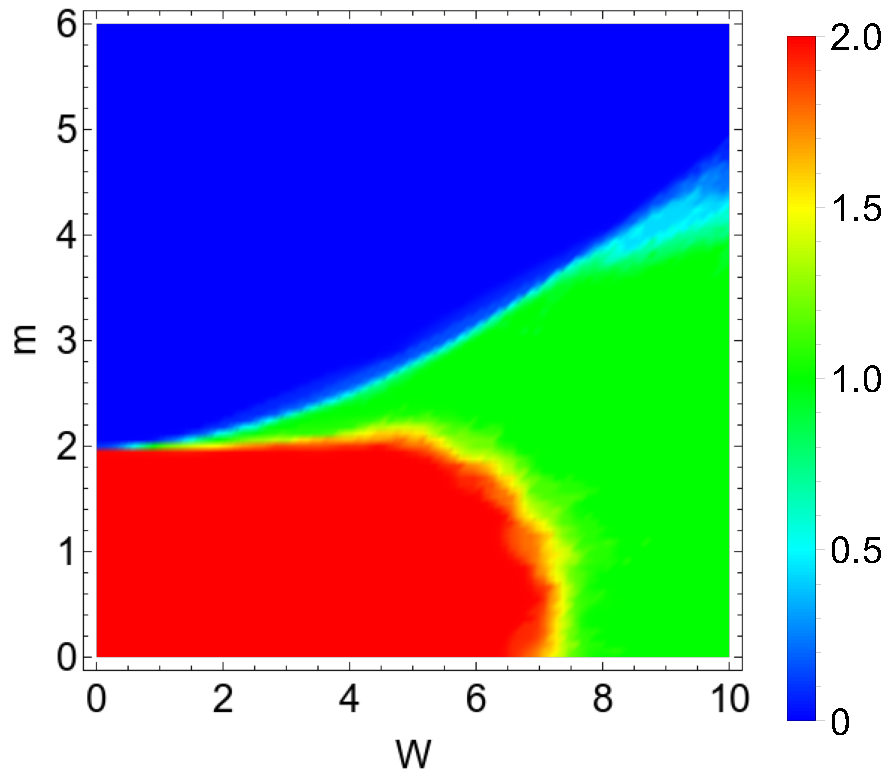
\includegraphics[width=45mm]{plotwinding.pdf}
		}		
	}\hspace{0mm}
	
	\makebox[0pt]{
		\subfloat[${\rm Log}_{10} (C \, {\rm mod} \, 1)$ ]{
			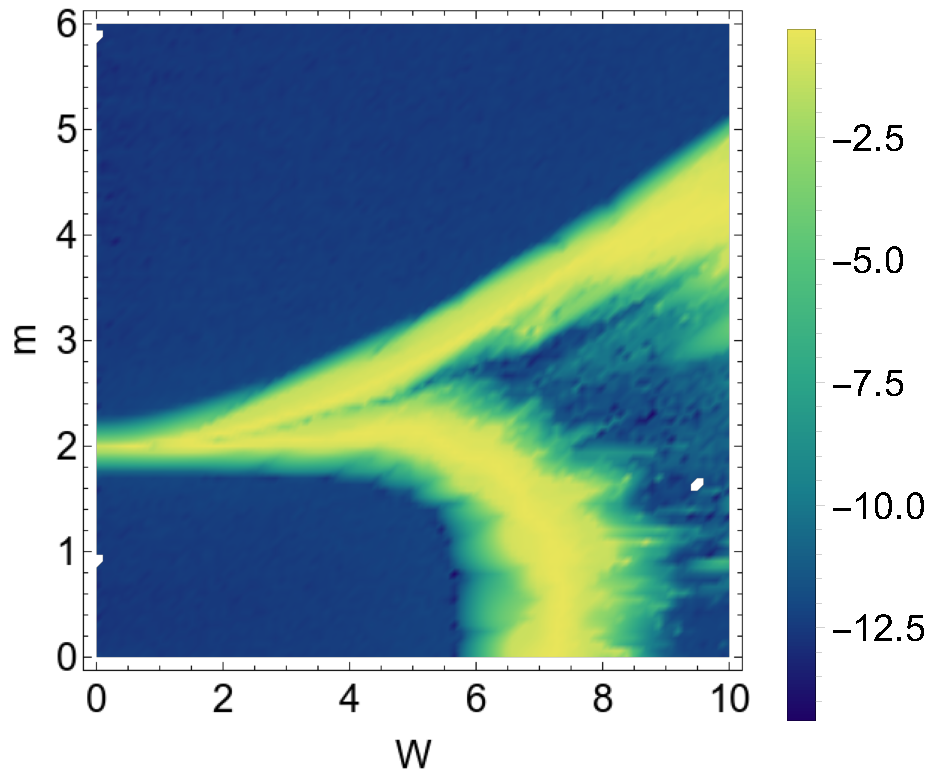
\includegraphics[width=45mm]{plotwindingerror.pdf}
		}
	}
	\caption{We compute (a)$\tilde{\mathcal{P}}_{\rm open}$, (b) $\nu$ and (c) error in the quantization of $\nu$ for the continuous line in the phase diagram, $t=1,t'=2$ and system size $L=400$. (a) is computed for $W=6$ showing that the branch cut is not affected by the disorder. (b) and (c) are computed for increasing disorder strength, showing a good quantization of the resulting winding number far from the transitions. }
	\label{winding}
\end{figure}



\subsubsection{$t' \neq 0$}

The analysis we did above of $\tpo$ for the SSH chain seems rather trivial as $\tpo$ does not seem to have more information than $\tilde{\mathcal{P}}$ modulo 1. This is no longer true when $t' \neq 0$ allowing for a $\nu = 2$ phase. In Fig.\ref{ssh_chern}.(c) we see $\tpo$ for the dotted cut in the phase diagram with an added symmetry breaking $\kappa$. We see clearly that $\tpo$ distinguishes between the $\nu=0$ and $\nu = 2$ phases. Similar to before, there is a gauge choice that makes $\tpo$ continuous in $\kappa$.
However, which gauge transformation does this is a priori not known, so in practice we can only compute the limit $\lim_{\kappa \rightarrow 0} \tpo$ in the original gauge.

Our expression for the Chern number \eqref{eq:Chern_number} is also valid without translational invariance. Consider now that we add disorder in the $t$ and $m$ parameters
\begin{align}
&t_i = t + \frac{W}{2} \omega_i \nonumber\\
&m_i = m + W \omega'_i
\end{align}
where $\omega_i$ and $\omega_i$ are randomly selected from $[-1/2,1/2]$. For very strong disorder, where the gap fills with states, the limit $\lim_{\kappa \rightarrow 0} \tilde{\mathcal{P}}_{\rm open}$ might become problematic as bulk states can cross $E=0$ as we tune $\kappa$ down. In order to avoid it we break chiral symmetry locally in the edge of the open chain so it only affects the zero modes. If any of the other states cross $E=0$ they do it in pairs such that $\tilde{\mathcal{P}}_{\rm open}$ is not affected by it. We show $\tilde{\mathcal{P}}_{\rm open}$ in Fig.\ref{winding}.(a) using the local symmetry breaking term for a strong disorder, $W=6t$, where the gap is indeed filled with states. In Fig.\ref{winding}.(b) we show $C$ for the continuous line in the phase diagram and increasing disorder strength. The Chern number as defined in \eqref{eq:Chern_number} indeed provides a topological invariant which can be compared with the winding number obtained in reference \cite{Song2014} for the same system. Note that for large enough systems the spectrum of $C_A$ is not affected by the local chiral symmetry breaking term other than the occupation of the zero-energy modes such that $C$ is still quantized, however near the transitions it is smoothen by the disorder average We show the error in the quantization of $C$ in figure \ref{winding}.(c) . 

\mariac{removed the paragraph about appendix D}
%\carlos{In Appendix D I give an expression for the winding number for flux insertion. However this expression seems problematic with a filled gap (Prodan refers to this). If we found an inhomogeneous term that induce a topological transition without filling the gap we can use this formula instead of comparing with the Prodan results, so we dont have to worry about the filled gap. 
%Furthermore I worked an expression for this winding number in terms of the correlation function, which I believe we might be able to relate to our $\chi$. However I can only do this on the open chain, where the winding number itself is not well-defined because the Hamiltonian is not invertible. We can do the trick of splitting the edge-modes and arguing that the winding number should not change by doing that because its a  bulk property, but I'm not too sure about that, so it would be better if we found a way of computing the winding number for open chains.   }

% - % - % - % - % - % - % - % - % - % - % - % - % - % - % - % - % - % - % - % - % - % - % - % - % - % - % - % - % - % - % - % - % - % - % - % - % - % 


\section{Conclusion}

It was previously known that the Zak phase, or the geometric phase for $U(1)$ flux insertion, was encoded in the many-body entanglement spectrum. Here we have shown how it is encoded in the single-body entanglement spectrum. This relation is simpler than the one involving the MBES and it provides more insight into the ES. Based on this method we show that one can obtain a polarization that is defined in the real axis. Although it is not gauge invariant it provides a method for computing Chern numbers for systems without translational invariance. We have also shown that the Chern number obtained this way is, for the system studied here, equivalent to the winding number.

\bibliography{references}	

	
\appendix

% - % - % - % - % - % - % - % - % - % - % - % - % - % - % - % - % - % - % - % - % - % - % - % - % - % - % - % - % - % - % - % - % - % - % - % - % - % 

\section{Computing the Zak phase from the Schmidt decomposition}\label{app:pollmann}

\maria{In this appendix, we review  how to compute the Zak phase from the Schmidt decomposition~\cite{Zaletel2014}and relate it to our own results}


Consider a closed chain of length $L$ and a bipartition into regions $A$, for $i\in [1,L/2]$, and $B$, for $i \in [L/2+1,L]$. Using a Schmidt decomposition the ground state gives
\begin{equation}
\ket{\Psi_C} = \sum_{p,q} s_p s'_q \ket{p,q}_A \ket{q,p}_B,
\end{equation}
The Schmidt indeces $p$ and $q$ label the fluctuations at the cuts in $i=1$ and $i=L/2$, respectively. The convention used for the states $\ket{p,q}_{R}$ is that the first (second) index labels the state near the left-most (right-most) region of $R$, where $R$ can be $A$ or $B$. Assuming the system is large enough compared with the correlation length the fluctuations across the two cuts are independent of each other. The reduced density matrix can be computed as
\begin{equation}
\rho_A = \sum_{p,q} s_p^2 s^{\prime \, 2}_q \ket{p,q}_{A}\bra{p,q}_A .
\end{equation}
As mentioned in section \ref{section:ES} it is fully determined by the correlation matrix $C_A$. In the state $\ket{p,q}_A$, the Schmidt index $p$ ($q$) labels a set of occupation numbers of the eigenstates of $C_A$ related to the cut at $i=1$ ($i=L/2$). we will refer to these subspaces of the Hilbert space as $A_L$ ($A_R$). Note that the remaining subspace $A_{\rm bulk}$ is composed of eigenstates that have eigenvalues $\xi = 0,1$. The eigenvalues of $\rho_A$, $\lambda_{pq}=s_p^2 s_q^{\prime \, 2}$ can be obtained as
\begin{align}
\lambda_{pq} =& \prod_{\mu \in A} (1-\xi_\mu)\left(\frac{\xi_\mu}{1-\xi_\mu}\right)^{n_\mu^{pq}} \\
=&\left(\prod_{\mu\in A_L} (1-\xi_\mu)\left(\frac{\xi_\mu}{1-\xi_\mu}\right)^{n_\mu^{p}} \right) \\
&\cross \left(\prod_{\nu \in A_R} (1-\xi_\nu)\left(\frac{\xi_\nu}{1-\xi_\nu}\right)^{n_\nu^{q}} \right) ,
\label{eq:Alexandrinata}
\end{align}
from which we identify 
\begin{align*}
&s_p^2 = \prod_{\mu\in A_L} (1-\xi_\mu)\left(\frac{\xi_\mu}{1-\xi_\mu}\right)^{n_\mu^{p}} \\
&s_q^{\prime 2} = \prod_{\nu \in A_R} (1-\xi_\nu)\left(\frac{\xi_\nu}{1-\xi_\nu}\right)^{n_\nu^{q}}.
\label{eq:spsq_A}
\end{align*}

We are now in position to introduce the $U(1)$ flux via a twisted boundary condition as
\begin{equation}
\ket{\Psi_0^\Phi} = \sum_{pq} s_p s_q' e^{-i\Phi N_{A_L}^p} \ket{p,q}_A \ket{q,p}_B,
\label{eq:Ground_state_flux}
\end{equation}
where $N_{A_L}^p = \sum_{\mu \in A_L}n_\mu^p$. As mentioned above, the label $p$ describes the set of occupation numbers $\{n_\mu^p\}$. Equation \eqref{eq:Ground_state_flux} means that an electron crossing the virtual cut at $i=1$ between region $B$ and $A_L$ will acquire a phase $-\Phi$, the convention on the sign is the same as the one used in reference \cite{Watanabe2018}. 

The polarization can be now computed as
\begin{align}
\tilde{\mathcal{P}} =& \int_0^{2\pi} \frac{d\Phi}{2\pi}i\bra{\Psi_0^\Phi}\partial_\Phi\ket{\Psi_0^\Phi} \\
=& \int_0^{2\pi} \frac{d\Phi}{2\pi}i\sum_{p,q} s_p^2 s_q^{\prime \, 2} e^{i\Phi N_{A_L}^p}\partial_{\Phi}e^{-i\Phi  N_{A_L}^p}\\
=&\int_0^{2\pi} \frac{d\Phi}{2\pi}\sum_{p,q} s_p^2 s_q^{\prime \, 2}  N_{A_L}^p\\
=&\sum_{p} s_p^2 \sum_{\mu \in A_L}n^p_\mu,
\end{align}
where we used that $\sum_q s_q^{\prime \,2} = 1$. Inserting now the expression for $s_p^2$ we obtain
\begin{align}
\tilde{\mathcal{P}}=&\sum_{\{n_{i \in A_L}\} = 0,1} \left(\sum_{j\in A_{L}} n_j \right) \left(\prod_{k\in A_L} \lambda_k \right),
\end{align} 
where we defined
\begin{equation}
\lambda_k = (1- \xi_k)\left(\frac{\xi_k}{1-\xi_k} \right)^{n_k}.
\end{equation}

If we expand the sum for one particular occupation number $n_p$ we have
\begin{align}
\tilde{\mathcal{P}} =& \sum_{\substack{\{n_{i \neq p \in A_L}\} = 0,1 \\ n_p=0}} \left(\sum_{j\neq p \in A_{L}} n_j \right) (1-\xi_p)\left(\prod_{k \neq p\in A_L} \lambda_k \right) \\
&+ \sum_{\substack{\{n_{i \neq p \in A_L}\} = 0,1 \\ n_p=0}} \left(\sum_{j\neq p \in A_{L}} n_j+1 \right)\xi_p \left(\prod_{k \neq p\in A_L} \lambda_k \right) \\
=& \sum_{\substack{\{n_{i \neq p \in A_L}\} = 0,1 }} \left(\sum_{j\neq p \in A_{L}} n_j \right) \left(\prod_{k \neq p\in A_L} \lambda_k \right) \\
&+ \xi_p \sum_{\substack{\{n_{i \neq p \in A_L}\} = 0,1 }} \left(\prod_{k \neq p\in A_L} \lambda_k \right) 
\end{align}
If we continue expanding the sum in the first term we will get terms like the second one for all the other $k\neq p$ eigenvalues. If we further expand the sum in the factor accompanying $\xi_p$ we have
\begin{align}
&(1-\xi_{p'})\sum_{\substack{\{n_{i \neq p,p' \in A_L}\} = 0,1 \\ n_{p'}=0}} \left(\prod_{k \neq p,p'\in A_L} \lambda_k\right) \\
&+ \xi_{p'}\sum_{\substack{\{n_{i \neq p,p' \in A_L}\} = 0,1 \\ n_{p'}=1}} \left(\prod_{k \neq p,p'\in A_L}\lambda_k\right) =1,
\end{align}
which we can see is $1$ if we continue this procedure for all other occupation numbers. Therefore in terms of the spectrum of $C_A$ the first term of the polarization greatly simplifies to 
\begin{align}
\tilde{\mathcal{P}} =& \sum_{p\in A_L}\xi_p  \quad {\rm mod}\, 1.
\end{align}
The subspace $A_L$ is not well-defined, as one can always include bulk modes. As a result the polarization obtained this way is defined only modulo 1. In practice we extend $A_L$ to include all eigenstates whose average position lies in the left half of $A$ and we finally get
\begin{align}
\tilde{\mathcal{P}} =& \sum_{i\in L}\xi_i \quad {\rm mod}\, 1.
\label{eq:polarization_left}
\end{align}

\section{Alternative expression for the correlation matrix}\label{app:CM}
In this appendix, we show how to express the correlation matrix in terms of the Hamiltonian, used in Eq.~\eqref{eq:corr_mat2}. 
We consider the generic, quadratic Hamiltonian in one dimension of Eq.~\ref{eq:quadr_Ham}, which is diagonalized by a unitary matrix $U$ with 
	\begin{align}\label{eq:D}
	H&=UDU^\dagger& \mbox{with } D=\mbox{diag}(E_{p\mu}).
	\end{align} 
In terms of the fermionic operators that diagonalize the Hamiltonian, 
\begin{align}
& \gamma_{i\alpha} = \sum_{j\beta}u_{j\beta}^{i\alpha \, \ast} c_{j\beta},
%& c_{i\alpha} = \sum_{j\beta} u^{j\beta}_{i\alpha} \gamma_{j\beta}
\end{align}
we find that the correlation matrix can be written as 
\begin{align}\label{eq:corr_mat}
C_{ij}^{\alpha \beta} =& \sum_{pq,\mu\nu} u^{q\nu }_{j\beta} u^{p\mu \, \ast}_{i\alpha} \expval{\gamma^\dagger_{p\mu} \gamma_{q\nu} }\nonumber \\
=&  \sum_{p\mu} u^{p\mu }_{j\beta} u^{p\mu \, \ast}_{i\alpha} \expval{\gamma^\dagger_{p\mu} \gamma_{p\mu} }\nonumber \\
=&  \sum_{p\mu} u^{p\mu }_{j\beta} u^{p\mu \, \ast}_{i\alpha} [1-{\rm sign}(E_{p\mu})]/2.
\end{align}
The first term of the last line is simply a kronecker delta between both sets of indices. 

The second term can be rewritten, using Eq.~\ref{eq:D}, as
\begin{align}
UD(\abs{D})^{-1}U^\dagger =& UDU^\dagger U(D^2)^{-1/2}U^\dagger
\end{align}
We can rewrite this expression further by noting that 
\begin{align}
[U (D^2)^{-1/2} U^\dagger]^2 =& U (D^2)^{-1/2} U^\dagger U  (D^2)^{-1/2} U^\dagger \nonumber\\
=&  U (D^2)^{-1/2}  (D^2)^{-1/2} U^\dagger \nonumber\\
=&  U (D^2)^{-1} U^\dagger \nonumber\\
=&  (U D^2 U^\dagger)^{-1}.
\end{align}
Therefore,
\begin{align*}
U (D^2)^{-1/2} U^\dagger =&(U D^2 U^\dagger)^{-1/2} 
\end{align*}
and we conclude that
\begin{align}\label{eq:UDDU}
UD(\abs{D})^{-1}U^\dagger =& UDU^\dagger(U D^2 U^\dagger)^{-1/2} \nonumber\\ 
=& H(H^2)^{-1/2}.
\end{align}
Combining Eq.s~\eqref{eq:corr_mat},  and \eqref{eq:UDDU}, we arrive at the final expression of the correlation matrix in Eq.~\eqref{eq:corr_mat2}. 

\section{Winding number in the SSH chain}
\label{appendix:winding_ssh}


Consider the Bloch Hamiltonian of the Rice-Mele model
\begin{equation}
H=\mqty(\kappa & f(k) \\ f^\dagger(k) & -\kappa),
\end{equation}
which can also be written as $H = \boldsymbol{h}\cdot \boldsymbol{\sigma}$
where 
\begin{align*}
\boldsymbol{h}=& ({\rm Re}[f(k)],-{\rm Im}[f(k)],\kappa) \\
=& \sqrt{\abs{f(k)}^2 +\kappa^2}(\sin(\theta)\cos(\phi),\sin(\theta)\sin(\phi),\cos(\theta))
\end{align*}
In the gauge where the second component of the eigenstates remains real they are given by
\begin{align}
&\ket{+}  = \frac{1}{N_+}\mqty(\cot(\theta/2)e^{-i\phi}\\ 1 )\\
&\ket{-}  =\frac{1}{N_-} \mqty(-\tan(\theta/2)e^{-i\phi}\\ 1),
\end{align}
where
\begin{align*}
&N_+ = \sqrt{1+\cot^2(\theta/2)} \\
&N_- = \sqrt{1+\tan^2(\theta/2)} .
\end{align*}
The Berry connections of the occupied state, $A_\lambda = \bra{-}\partial_\lambda \ket{-}$, can be obtained as
\begin{align*}
A_{\lambda}=& i\frac{\cos(\theta)-1}{2}\partial_q \phi \\
=&i\frac{\cos(\theta)-1}{2} \cos(\phi)^2 \partial_q  \tan(\phi) \\
=&\frac{i}{2}\left(\frac{\kappa}{\sqrt{\abs{f(k)}^2+\kappa^2}}-1\right) \left( \frac{\Re [f(k)]}{\abs{f(k)}}\right)^2 \partial_\lambda  \left( -\frac{\Im [f(k)]}{\Re [f(k)]} \right) \\
=&\frac{-1}{2}\left(\frac{\kappa}{\sqrt{\abs{f(k)}^2+\kappa^2}}-1\right) \frac{f(k)^\dagger \partial_\lambda f(k)-f(k)\partial_\lambda f(k)^\dagger}{2\abs{f(k)}^2}
\end{align*}
The Berry connection with respect to momentum gives
\begin{equation}
A_k = \frac{it [t+m \cos(k)][\kappa - \sqrt{\kappa^2+m^2+t^2+2mt \cos(k)}]}{2[m^2+t^2+2mt\cos(k)]\sqrt{\kappa^2+m^2+t^2+2mt \cos(k)}},
\end{equation}
and the resulting Zak phase can be seen in Fig.\ref{fig:ssh_zak}, which presents a branch cut for $m=0,\kappa<0$ for this particular gauge.


\begin{figure}[t]
	\centering
	\includegraphics[width=50mm]{sshwindinganalytical.pdf}
	\caption{$\gamma/2\pi$ obtained in the smooth gauge that provides the winding number in the chiral symmetric limit.}
	\label{fig:ssh_zak}
\end{figure}

Note that in the chiral symmetric case, for $\kappa = 0$, the Zak phase is
\begin{align*}
\gamma =& \int_0^{2\pi} dk\,\frac{1}{2}\frac{f(k)^\dagger \partial_k f(k)-f(k)\partial_k f(k)^\dagger}{2\abs{f(k)}^2} \\
=& \int_0^{2\pi} dk\,\frac{1}{2}q(k)^\dagger \partial_k q(k),
\end{align*}
where $q(k) = f(k)/\abs{f(k)}$. This is nothing else than the winding number \cite{ryu2010topological}. 

Consider now that we parametrize a loop in parameter space as $m=1-\cos(\theta),\kappa = \sin(\theta)$.

\mariac{removed appendix D}
%\section{Twisted boundary condition Winding number}
%\carlos{Work in progress}
%For a system with chiral symmetry the Hamiltonian can be written in some basis as
%\begin{equation}
%H = \mqty(0 & h \\ h^\dagger & 0),
%\end{equation}
%where $h$ is in general a matrix. In translationally invariant systems the winding number is defined as 
%\begin{equation}
%\nu = -i\int_0^{2\pi} \frac{dk}{2\pi} {\rm Tr}[h(k)^{-1} \partial_k h(k)],
%\label{eq:winding_k}
%\end{equation}
%where $h(k)$ is the off-diagonal block of the Bloch Hamiltonian. In systems without translational invariance, one can similarly define the winding number
%\begin{equation}
%\nu = -i\int_0^{2\pi} \frac{d\Phi}{2\pi} {\rm Tr}[h(\Phi)^{-1} \partial_\Phi h(\Phi)],
%\label{eq:winding_flux}
%\end{equation}
%for a $U(1)$ flux introduced (\carlos{I have only found a similar expression in the context of non-hermitian systems \cite{Gong2018}, but I assume this is the expression Prodan refers to. It gives the correct results in translationally invariant systems, however it is very unpractical.}). Note that a generalization of \eqref{eq:winding_k} to position space has also been developed which not necesseraly gives the same results as \eqref{eq:winding_flux} (\carlos{The only comparison is in the Prodan paper where they talk about practical numerical implementations but don't adress if both formulations are equivalent.}) Both formulations however reduce to \eqref{eq:winding_k} for translationally invariant systems \cite{Gong2018}.  In the following we will omit the flux parameter for simplicity.
%
%Note that the winding number can also be expressed in terms of the flat-band Hamiltonian
%\begin{align*}
%Q =& H (H^2)^{-1/2} \\
%=& \mqty(0 & q \\ q^\dagger & 0).
%\end{align*}
%Note that since $Q$ only has eigenvalues $\pm 1 $ , $Q^2 = \mathbb{I}$ and therefore $q^\dagger = q^{-1}$. We can therefore write
%\begin{equation}
%\nu = -i\int_0^{2\pi} \frac{d\Phi}{2\pi} {\rm Tr}[q^\dagger \partial_\Phi q].
%\end{equation}
%In this basis the chiral symmetry operator is given by $S = \sigma_z \otimes \mathbb{I}$ such that the winding number can be expressed in terms of the full flat-band Hamiltonian as
%\begin{align}
%\nu =& \frac{i}{2}\int_0^{2\pi} \frac{d\Phi}{2\pi} {\rm Tr}[S Q^\dagger \partial_\Phi Q] \\
%=& \frac{i}{2}\int_0^{2\pi} \frac{d\Phi}{2\pi} \left({\rm Tr}[q \partial_\Phi q^\dagger]-{\rm Tr}[q^\dagger \partial_\Phi q] \right)\\
%=& -i\int_0^{2\pi} \frac{d\Phi}{2\pi} {\rm Tr}[q^\dagger \partial_\Phi q] 
%\end{align}
%where in the last step we use the fact that the winding number is a real number. We can now write the winding number in terms of the correlation matrix
%\begin{align}
%\nu =& \frac{i}{2}\int_0^{2\pi} \frac{d\Phi}{2\pi} {\rm Tr}[S (1-2C) \partial_\Phi (1-2C)] \\
%=& -i\int_0^{2\pi} \frac{d\Phi}{2\pi} {\rm Tr}[S (1-2C) \partial_\Phi C] .
%\end{align}
%Introducing the flux via twisted boundary conditions allows us to easily construct the ground state with flux in the case of the open chain \eqref{eq:gauge}, therefore we will employ this gauge to compute the correlation matrix. The correlation matrix can be written in position space as
%\begin{equation}
%C = \mqty(C_A & C_{AB} \\ C_{AB}^\dagger & C_B),
%\end{equation}
%where in this basis, assuming $S$ is a local symmetry it is also diagonal. Note that the flux will only appear in the off-diagonal blocks $C_{AB}$ and therefore the first term in the trace above will vanish, leaving the winding number as
%\begin{align}
%\nu =&  -i\int_0^{2\pi} \frac{d\Phi}{2\pi} {\rm Tr}[S C \partial_\Phi C] \\
%=&  -i\int_0^{2\pi} \frac{d\Phi}{2\pi} \left( {\rm Tr}[S C_{AB} \partial_\Phi C_{AB}^\dagger]+{\rm Tr}[S C_{AB}^\dagger \partial_\Phi C_{AB}] \right)
%\end{align}
%We can not explicitely construct the correlation matrix with flux as
%\begin{align*}
%C_{ij}^\Phi =& \bra{\tilde{\Psi}_{0,{\rm open}}^\Phi}c_i^\dagger c_j \ket{\tilde{\Psi}_{0,{\rm open}}^\Phi} \\
%=&\bra{\tilde{\Psi}_{0,{\rm open}}^0}e^{i\Phi \hat{N}_A} c_i^\dagger c_j e^{-i\Phi \hat{N}_A}\ket{\tilde{\Psi}_{0,{\rm open}}^0} .
%\end{align*}
%Depending on if $i,j$ belong to $A$ or not, commuting the exponentials will leave additional factors or not, resulting in
%\begin{align*}
%C^\Phi = \mqty(C_A^0 & e^{i\Phi} C_{AB}^0 \\e^{-i\Phi} C_{AB}^{0\,\dagger} &C_B^{0}),
%\end{align*}
%where we have made explicit the flux dependence. The winding number is then
%\begin{align}
%\nu =&  -i\int_0^{2\pi} \frac{d\Phi}{2\pi} {\rm Tr}[S C^\Phi \partial_\Phi C^\Phi] \\
%=&  -i\int_0^{2\pi} \frac{d\Phi}{2\pi} \left( {\rm Tr}[-iS C_{AB}^0 C_{AB}^{0\,\dagger}]+{\rm Tr}[iS C_{AB}^{0\,^\dagger} C_{AB}^0] \right) \\
%=&  {\rm Tr}[S C_B^0(1-C_B^0)]-{\rm Tr}[S C_A^0(1-C_A^0)] 
%\end{align}
%where in the last step we use one of the properties of the correlation function stemming from $C^2 = C$. (\carlos{So far this expression gives the correct result for translationally invariant systems however one needs to do the trick of breaking chiral symmetry slightly. However, unlike with $\tilde{\mathcal{P}}$ this expression is not discontinuous at $\kappa = 0$. })
%


\end{document}